\documentclass{book}
\usepackage[a4paper,top=2.5cm,bottom=2.5cm,left=2.5cm,right=2.5cm]{geometry}
\usepackage{makeidx}
\usepackage{natbib}
\usepackage{graphicx}
\usepackage{multicol}
\usepackage{float}
\usepackage{listings}
\usepackage{color}
\usepackage{ifthen}
\usepackage[table]{xcolor}
\usepackage{textcomp}
\usepackage{alltt}
\usepackage{ifpdf}
\ifpdf
\usepackage[pdftex,
            pagebackref=true,
            colorlinks=true,
            linkcolor=blue,
            unicode
           ]{hyperref}
\else
\usepackage[ps2pdf,
            pagebackref=true,
            colorlinks=true,
            linkcolor=blue,
            unicode
           ]{hyperref}
\usepackage{pspicture}
\fi
\usepackage[utf8]{inputenc}
\usepackage{mathptmx}
\usepackage[scaled=.90]{helvet}
\usepackage{courier}
\usepackage{sectsty}
\usepackage{amssymb}
\usepackage[titles]{tocloft}
\usepackage{doxygen}
\lstset{language=C++,inputencoding=utf8,basicstyle=\footnotesize,breaklines=true,breakatwhitespace=true,tabsize=8,numbers=left }
\makeindex
\setcounter{tocdepth}{3}
\renewcommand{\footrulewidth}{0.4pt}
\renewcommand{\familydefault}{\sfdefault}
\hfuzz=15pt
\setlength{\emergencystretch}{15pt}
\hbadness=750
\tolerance=750
\begin{document}
\hypersetup{pageanchor=false,citecolor=blue}
\begin{titlepage}
\vspace*{7cm}
\begin{center}
{\Large Collider++ }\\
\vspace*{1cm}
{\large Generated by Doxygen 1.8.3.1-20130209}\\
\vspace*{0.5cm}
{\small Sat Mar 30 2013 19:06:03}\\
\end{center}
\end{titlepage}
\clearemptydoublepage
\pagenumbering{roman}
\tableofcontents
\clearemptydoublepage
\pagenumbering{arabic}
\hypersetup{pageanchor=true,citecolor=blue}
\chapter{Hierarchical Index}
\section{Class Hierarchy}
This inheritance list is sorted roughly, but not completely, alphabetically\-:\begin{DoxyCompactList}
\item \contentsline{section}{sc\-:\-:Buffer}{\pageref{classsc_1_1Buffer}}{}
\item \contentsline{section}{sc\-:\-:Bus}{\pageref{classsc_1_1Bus}}{}
\item \contentsline{section}{sc\-:\-:Node}{\pageref{classsc_1_1Node}}{}
\begin{DoxyCompactList}
\item \contentsline{section}{sc\-:\-:Group}{\pageref{classsc_1_1Group}}{}
\begin{DoxyCompactList}
\item \contentsline{section}{sc\-:\-:Root\-Node}{\pageref{classsc_1_1RootNode}}{}
\end{DoxyCompactList}
\item \contentsline{section}{sc\-:\-:Synth}{\pageref{classsc_1_1Synth}}{}
\end{DoxyCompactList}
\item \contentsline{section}{sc\-:\-:S\-C\-Server}{\pageref{classsc_1_1SCServer}}{}
\item \contentsline{section}{sc\-:\-:Sound}{\pageref{classsc_1_1Sound}}{}
\end{DoxyCompactList}

\chapter{Class Index}
\section{Class List}
Here are the classes, structs, unions and interfaces with brief descriptions\-:\begin{DoxyCompactList}
\item\contentsline{section}{\hyperlink{classColliderPlusPlus_1_1Buffer}{Collider\-Plus\-Plus\-::\-Buffer} \\*This class represents a client-\/side version of a server buffer }{\pageref{classColliderPlusPlus_1_1Buffer}}{}
\item\contentsline{section}{\hyperlink{classColliderPlusPlus_1_1Bus}{Collider\-Plus\-Plus\-::\-Bus} }{\pageref{classColliderPlusPlus_1_1Bus}}{}
\item\contentsline{section}{\hyperlink{classColliderPlusPlus_1_1Client__Server}{Collider\-Plus\-Plus\-::\-Client\-\_\-\-Server} \\*This class represents a client-\/side version of scsynth, the Super\-Collider audio server }{\pageref{classColliderPlusPlus_1_1Client__Server}}{}
\item\contentsline{section}{\hyperlink{classColliderPlusPlus_1_1Group}{Collider\-Plus\-Plus\-::\-Group} \\*This class represents a client-\/side version of a server group }{\pageref{classColliderPlusPlus_1_1Group}}{}
\item\contentsline{section}{\hyperlink{classColliderPlusPlus_1_1Node}{Collider\-Plus\-Plus\-::\-Node} \\*This class represents a client-\/side version of a server node (\hyperlink{classColliderPlusPlus_1_1Synth}{Synth} or \hyperlink{classColliderPlusPlus_1_1Group}{Group}) }{\pageref{classColliderPlusPlus_1_1Node}}{}
\item\contentsline{section}{\hyperlink{classColliderPlusPlus_1_1RootNode}{Collider\-Plus\-Plus\-::\-Root\-Node} \\*This class represents a client-\/side version of a server root node }{\pageref{classColliderPlusPlus_1_1RootNode}}{}
\item\contentsline{section}{\hyperlink{classColliderPlusPlus_1_1Sound}{Collider\-Plus\-Plus\-::\-Sound} \\*This class represents a user manipulable Soundfile Player, essentially mirroring the O\-A\-S class of the same name by Shreenidhi Chowkwale  \href{https://github.com/CalVR/Open-Audio-Server/blob/master/client/src/Sound.h}{\tt https\-://github.\-com/\-Cal\-V\-R/\-Open-\/\-Audio-\/\-Server/blob/master/client/src/\-Sound.\-h} }{\pageref{classColliderPlusPlus_1_1Sound}}{}
\item\contentsline{section}{\hyperlink{classColliderPlusPlus_1_1Synth}{Collider\-Plus\-Plus\-::\-Synth} \\*This class represents a client-\/side version of a server synth }{\pageref{classColliderPlusPlus_1_1Synth}}{}
\end{DoxyCompactList}

\chapter{File Index}
\section{File List}
Here is a list of all documented files with brief descriptions\-:\begin{DoxyCompactList}
\item\contentsline{section}{include/\hyperlink{Buffer_8hpp}{Buffer.\-hpp} \\*Header file for \hyperlink{Buffer_8hpp}{Buffer.\-hpp} }{\pageref{Buffer_8hpp}}{}
\item\contentsline{section}{include/\hyperlink{Bus_8hpp}{Bus.\-hpp} \\*Header file for \hyperlink{Bus_8hpp}{Bus.\-hpp} }{\pageref{Bus_8hpp}}{}
\item\contentsline{section}{include/{\bfseries libcollider.\-hpp} }{\pageref{libcollider_8hpp}}{}
\item\contentsline{section}{include/\hyperlink{Node_8hpp}{Node.\-hpp} \\*Header file for \hyperlink{Node_8hpp}{Node.\-hpp} }{\pageref{Node_8hpp}}{}
\item\contentsline{section}{include/\hyperlink{SCServer_8hpp}{S\-C\-Server.\-hpp} \\*Header file for \hyperlink{SCServer_8hpp}{S\-C\-Server.\-hpp} }{\pageref{SCServer_8hpp}}{}
\item\contentsline{section}{include/\hyperlink{Sound_8hpp}{Sound.\-hpp} \\*Header file for \hyperlink{Sound_8hpp}{Sound.\-hpp} }{\pageref{Sound_8hpp}}{}
\end{DoxyCompactList}

\chapter{Class Documentation}
\hypertarget{classColliderPlusPlus_1_1Buffer}{\section{Collider\-Plus\-Plus\-:\-:Buffer Class Reference}
\label{classColliderPlusPlus_1_1Buffer}\index{Collider\-Plus\-Plus\-::\-Buffer@{Collider\-Plus\-Plus\-::\-Buffer}}
}


This class represents a client-\/side version of a server buffer.  




{\ttfamily \#include $<$Buffer.\-hpp$>$}

\subsection*{Public Member Functions}
\begin{DoxyCompactItemize}
\item 
\hypertarget{classColliderPlusPlus_1_1Buffer_aac5d271b57c8b6410b790794cfb790e1}{\hyperlink{classColliderPlusPlus_1_1Buffer_aac5d271b57c8b6410b790794cfb790e1}{Buffer} ()}\label{classColliderPlusPlus_1_1Buffer_aac5d271b57c8b6410b790794cfb790e1}

\begin{DoxyCompactList}\small\item\em Default Constructor. \end{DoxyCompactList}\item 
\hyperlink{classColliderPlusPlus_1_1Buffer_a253743cd16ea0a2579575dd9472a967d}{Buffer} (\hyperlink{classColliderPlusPlus_1_1Client__Server}{Client\-\_\-\-Server} $\ast$cs, int buf\-Num)
\item 
\hypertarget{classColliderPlusPlus_1_1Buffer_a62178f1cb35c5654c0b16d78526de7e8}{\hyperlink{classColliderPlusPlus_1_1Buffer_a62178f1cb35c5654c0b16d78526de7e8}{$\sim$\-Buffer} ()}\label{classColliderPlusPlus_1_1Buffer_a62178f1cb35c5654c0b16d78526de7e8}

\begin{DoxyCompactList}\small\item\em Destructor. \end{DoxyCompactList}\item 
int \hyperlink{classColliderPlusPlus_1_1Buffer_a6d2eb844b20eb62158d5d77bcb5d568c}{\-\_\-get\-Buf\-Num} () const 
\item 
int \hyperlink{classColliderPlusPlus_1_1Buffer_adbd84c84d0c13d9dcc96e36edce17448}{\-\_\-get\-Frame\-Num} () const 
\item 
int \hyperlink{classColliderPlusPlus_1_1Buffer_a1eca16cfed94680f3a14adcd4dfe42c9}{\-\_\-get\-Chan\-Num} () const 
\item 
int \hyperlink{classColliderPlusPlus_1_1Buffer_a6887218a82f341f668117cd24548921a}{\-\_\-get\-Samp\-Rate} () const 
\item 
const std\-::string \& \hyperlink{classColliderPlusPlus_1_1Buffer_a94c409839084712d7cc10fd46e520d68}{\-\_\-get\-File\-Path} () const 
\item 
bool \hyperlink{classColliderPlusPlus_1_1Buffer_abe0bd6783d6619ad9df0b5b6cd194d73}{\-\_\-get\-Manually\-Freed} () const 
\item 
void \hyperlink{classColliderPlusPlus_1_1Buffer_af0248190521ac9b499da2595f5519b12}{\-\_\-alloc} (int num\-Frames, int num\-Channels)
\item 
void \hyperlink{classColliderPlusPlus_1_1Buffer_acdb1aca3342219a321ff61645de4551f}{\-\_\-free} ()
\item 
void \hyperlink{classColliderPlusPlus_1_1Buffer_a15072b705358d59e252e1f6d515e3b94}{\-\_\-query} ()
\item 
void \hyperlink{classColliderPlusPlus_1_1Buffer_a0cbb99a9823f18b151f7f7da4bcf56a7}{\-\_\-alloc\-Read} (const std\-::string \&file\-Path, int start\-File\-Frame=0, int num\-Frames=-\/1)
\end{DoxyCompactItemize}


\subsection{Detailed Description}
This class represents a client-\/side version of a server buffer. 

\subsection{Constructor \& Destructor Documentation}
\hypertarget{classColliderPlusPlus_1_1Buffer_a253743cd16ea0a2579575dd9472a967d}{\index{Collider\-Plus\-Plus\-::\-Buffer@{Collider\-Plus\-Plus\-::\-Buffer}!Buffer@{Buffer}}
\index{Buffer@{Buffer}!ColliderPlusPlus::Buffer@{Collider\-Plus\-Plus\-::\-Buffer}}
\subsubsection[{Buffer}]{\setlength{\rightskip}{0pt plus 5cm}Collider\-Plus\-Plus\-::\-Buffer\-::\-Buffer (
\begin{DoxyParamCaption}
\item[{{\bf Client\-\_\-\-Server} $\ast$}]{cs, }
\item[{int}]{buf\-Num}
\end{DoxyParamCaption}
)}}\label{classColliderPlusPlus_1_1Buffer_a253743cd16ea0a2579575dd9472a967d}
Create a \hyperlink{classColliderPlusPlus_1_1Buffer}{Buffer} with buffer number specified by buf\-Num parameter 
\begin{DoxyParams}[1]{Parameters}
\mbox{\tt in}  & {\em \hyperlink{classColliderPlusPlus_1_1Client__Server}{Client\-\_\-\-Server}} & instance \\
\hline
\mbox{\tt in}  & {\em int} & \hyperlink{classColliderPlusPlus_1_1Buffer}{Buffer} Number \\
\hline
\end{DoxyParams}


\subsection{Member Function Documentation}
\hypertarget{classColliderPlusPlus_1_1Buffer_af0248190521ac9b499da2595f5519b12}{\index{Collider\-Plus\-Plus\-::\-Buffer@{Collider\-Plus\-Plus\-::\-Buffer}!\-\_\-alloc@{\-\_\-alloc}}
\index{\-\_\-alloc@{\-\_\-alloc}!ColliderPlusPlus::Buffer@{Collider\-Plus\-Plus\-::\-Buffer}}
\subsubsection[{\-\_\-alloc}]{\setlength{\rightskip}{0pt plus 5cm}void Collider\-Plus\-Plus\-::\-Buffer\-::\-\_\-alloc (
\begin{DoxyParamCaption}
\item[{int}]{num\-Frames, }
\item[{int}]{num\-Channels}
\end{DoxyParamCaption}
)}}\label{classColliderPlusPlus_1_1Buffer_af0248190521ac9b499da2595f5519b12}
Command server to allocate memory for this \hyperlink{classColliderPlusPlus_1_1Buffer}{Buffer} 
\begin{DoxyParams}[1]{Parameters}
\mbox{\tt in}  & {\em Client\-\_\-\-Server\&} & \hyperlink{classColliderPlusPlus_1_1Client__Server}{Client\-\_\-\-Server} instance \\
\hline
\mbox{\tt in}  & {\em int} & Number of Sample Frames \\
\hline
\mbox{\tt in}  & {\em int} & Number of Channels \\
\hline
\end{DoxyParams}
\hypertarget{classColliderPlusPlus_1_1Buffer_a0cbb99a9823f18b151f7f7da4bcf56a7}{\index{Collider\-Plus\-Plus\-::\-Buffer@{Collider\-Plus\-Plus\-::\-Buffer}!\-\_\-alloc\-Read@{\-\_\-alloc\-Read}}
\index{\-\_\-alloc\-Read@{\-\_\-alloc\-Read}!ColliderPlusPlus::Buffer@{Collider\-Plus\-Plus\-::\-Buffer}}
\subsubsection[{\-\_\-alloc\-Read}]{\setlength{\rightskip}{0pt plus 5cm}void Collider\-Plus\-Plus\-::\-Buffer\-::\-\_\-alloc\-Read (
\begin{DoxyParamCaption}
\item[{const std\-::string \&}]{file\-Path, }
\item[{int}]{start\-File\-Frame = {\ttfamily 0}, }
\item[{int}]{num\-Frames = {\ttfamily -\/1}}
\end{DoxyParamCaption}
)}}\label{classColliderPlusPlus_1_1Buffer_a0cbb99a9823f18b151f7f7da4bcf56a7}
Command server to load specified Soundfile into \hyperlink{classColliderPlusPlus_1_1Buffer}{Buffer} and allocate just enough space for the Soundfile with the given offset specified by start\-File\-Frame 
\begin{DoxyParams}[1]{Parameters}
\mbox{\tt in}  & {\em Client\-\_\-\-Server\&} & \hyperlink{classColliderPlusPlus_1_1Client__Server}{Client\-\_\-\-Server} instance \\
\hline
\mbox{\tt in}  & {\em const} & std\-::string\& Soundfile Path \\
\hline
\mbox{\tt in}  & {\em int} & Read file from this sample \\
\hline
\mbox{\tt in}  & {\em int} & Number of Sample Frames to allocate, -\/1 loads whole Soundfile \\
\hline
\end{DoxyParams}
\hypertarget{classColliderPlusPlus_1_1Buffer_acdb1aca3342219a321ff61645de4551f}{\index{Collider\-Plus\-Plus\-::\-Buffer@{Collider\-Plus\-Plus\-::\-Buffer}!\-\_\-free@{\-\_\-free}}
\index{\-\_\-free@{\-\_\-free}!ColliderPlusPlus::Buffer@{Collider\-Plus\-Plus\-::\-Buffer}}
\subsubsection[{\-\_\-free}]{\setlength{\rightskip}{0pt plus 5cm}void Collider\-Plus\-Plus\-::\-Buffer\-::\-\_\-free (
\begin{DoxyParamCaption}
{}
\end{DoxyParamCaption}
)}}\label{classColliderPlusPlus_1_1Buffer_acdb1aca3342219a321ff61645de4551f}
Command server to free memory associated with this \hyperlink{classColliderPlusPlus_1_1Buffer}{Buffer} 
\begin{DoxyParams}[1]{Parameters}
\mbox{\tt in}  & {\em Client\-\_\-\-Server\&} & \hyperlink{classColliderPlusPlus_1_1Client__Server}{Client\-\_\-\-Server} instance \\
\hline
\end{DoxyParams}
\hypertarget{classColliderPlusPlus_1_1Buffer_a6d2eb844b20eb62158d5d77bcb5d568c}{\index{Collider\-Plus\-Plus\-::\-Buffer@{Collider\-Plus\-Plus\-::\-Buffer}!\-\_\-get\-Buf\-Num@{\-\_\-get\-Buf\-Num}}
\index{\-\_\-get\-Buf\-Num@{\-\_\-get\-Buf\-Num}!ColliderPlusPlus::Buffer@{Collider\-Plus\-Plus\-::\-Buffer}}
\subsubsection[{\-\_\-get\-Buf\-Num}]{\setlength{\rightskip}{0pt plus 5cm}int Collider\-Plus\-Plus\-::\-Buffer\-::\-\_\-get\-Buf\-Num (
\begin{DoxyParamCaption}
{}
\end{DoxyParamCaption}
) const\hspace{0.3cm}{\ttfamily [inline]}}}\label{classColliderPlusPlus_1_1Buffer_a6d2eb844b20eb62158d5d77bcb5d568c}
Returns this \hyperlink{classColliderPlusPlus_1_1Buffer}{Buffer}'s number as an int \begin{DoxyReturn}{Returns}
int \hyperlink{classColliderPlusPlus_1_1Buffer}{Buffer} Number 
\end{DoxyReturn}
\hypertarget{classColliderPlusPlus_1_1Buffer_a1eca16cfed94680f3a14adcd4dfe42c9}{\index{Collider\-Plus\-Plus\-::\-Buffer@{Collider\-Plus\-Plus\-::\-Buffer}!\-\_\-get\-Chan\-Num@{\-\_\-get\-Chan\-Num}}
\index{\-\_\-get\-Chan\-Num@{\-\_\-get\-Chan\-Num}!ColliderPlusPlus::Buffer@{Collider\-Plus\-Plus\-::\-Buffer}}
\subsubsection[{\-\_\-get\-Chan\-Num}]{\setlength{\rightskip}{0pt plus 5cm}int Collider\-Plus\-Plus\-::\-Buffer\-::\-\_\-get\-Chan\-Num (
\begin{DoxyParamCaption}
{}
\end{DoxyParamCaption}
) const\hspace{0.3cm}{\ttfamily [inline]}}}\label{classColliderPlusPlus_1_1Buffer_a1eca16cfed94680f3a14adcd4dfe42c9}
Returns this \hyperlink{classColliderPlusPlus_1_1Buffer}{Buffer}'s channel count as an int \begin{DoxyReturn}{Returns}
int \hyperlink{classColliderPlusPlus_1_1Buffer}{Buffer} channel count 
\end{DoxyReturn}
\hypertarget{classColliderPlusPlus_1_1Buffer_a94c409839084712d7cc10fd46e520d68}{\index{Collider\-Plus\-Plus\-::\-Buffer@{Collider\-Plus\-Plus\-::\-Buffer}!\-\_\-get\-File\-Path@{\-\_\-get\-File\-Path}}
\index{\-\_\-get\-File\-Path@{\-\_\-get\-File\-Path}!ColliderPlusPlus::Buffer@{Collider\-Plus\-Plus\-::\-Buffer}}
\subsubsection[{\-\_\-get\-File\-Path}]{\setlength{\rightskip}{0pt plus 5cm}const std\-::string\& Collider\-Plus\-Plus\-::\-Buffer\-::\-\_\-get\-File\-Path (
\begin{DoxyParamCaption}
{}
\end{DoxyParamCaption}
) const\hspace{0.3cm}{\ttfamily [inline]}}}\label{classColliderPlusPlus_1_1Buffer_a94c409839084712d7cc10fd46e520d68}
Returns the file path of this \hyperlink{classColliderPlusPlus_1_1Buffer}{Buffer}'s loaded soundfile \begin{DoxyReturn}{Returns}
const std\-::string\& Soundfile Path 
\end{DoxyReturn}
\hypertarget{classColliderPlusPlus_1_1Buffer_adbd84c84d0c13d9dcc96e36edce17448}{\index{Collider\-Plus\-Plus\-::\-Buffer@{Collider\-Plus\-Plus\-::\-Buffer}!\-\_\-get\-Frame\-Num@{\-\_\-get\-Frame\-Num}}
\index{\-\_\-get\-Frame\-Num@{\-\_\-get\-Frame\-Num}!ColliderPlusPlus::Buffer@{Collider\-Plus\-Plus\-::\-Buffer}}
\subsubsection[{\-\_\-get\-Frame\-Num}]{\setlength{\rightskip}{0pt plus 5cm}int Collider\-Plus\-Plus\-::\-Buffer\-::\-\_\-get\-Frame\-Num (
\begin{DoxyParamCaption}
{}
\end{DoxyParamCaption}
) const\hspace{0.3cm}{\ttfamily [inline]}}}\label{classColliderPlusPlus_1_1Buffer_adbd84c84d0c13d9dcc96e36edce17448}
Returns this \hyperlink{classColliderPlusPlus_1_1Buffer}{Buffer}'s sample frame count as an int \begin{DoxyReturn}{Returns}
int \hyperlink{classColliderPlusPlus_1_1Buffer}{Buffer} sample frame count 
\end{DoxyReturn}
\hypertarget{classColliderPlusPlus_1_1Buffer_abe0bd6783d6619ad9df0b5b6cd194d73}{\index{Collider\-Plus\-Plus\-::\-Buffer@{Collider\-Plus\-Plus\-::\-Buffer}!\-\_\-get\-Manually\-Freed@{\-\_\-get\-Manually\-Freed}}
\index{\-\_\-get\-Manually\-Freed@{\-\_\-get\-Manually\-Freed}!ColliderPlusPlus::Buffer@{Collider\-Plus\-Plus\-::\-Buffer}}
\subsubsection[{\-\_\-get\-Manually\-Freed}]{\setlength{\rightskip}{0pt plus 5cm}bool Collider\-Plus\-Plus\-::\-Buffer\-::\-\_\-get\-Manually\-Freed (
\begin{DoxyParamCaption}
{}
\end{DoxyParamCaption}
) const\hspace{0.3cm}{\ttfamily [inline]}}}\label{classColliderPlusPlus_1_1Buffer_abe0bd6783d6619ad9df0b5b6cd194d73}
Returns true if the \hyperlink{classColliderPlusPlus_1_1Node}{Node} was freed from the server by calling \hyperlink{classColliderPlusPlus_1_1Buffer_acdb1aca3342219a321ff61645de4551f}{\-\_\-free()} B\-E\-F\-O\-R\-E the destructor of this \hyperlink{classColliderPlusPlus_1_1Node}{Node} is called \begin{DoxyReturn}{Returns}
true if freed from server with \hyperlink{classColliderPlusPlus_1_1Buffer_acdb1aca3342219a321ff61645de4551f}{\-\_\-free()} prior to destruction 
\end{DoxyReturn}
\hypertarget{classColliderPlusPlus_1_1Buffer_a6887218a82f341f668117cd24548921a}{\index{Collider\-Plus\-Plus\-::\-Buffer@{Collider\-Plus\-Plus\-::\-Buffer}!\-\_\-get\-Samp\-Rate@{\-\_\-get\-Samp\-Rate}}
\index{\-\_\-get\-Samp\-Rate@{\-\_\-get\-Samp\-Rate}!ColliderPlusPlus::Buffer@{Collider\-Plus\-Plus\-::\-Buffer}}
\subsubsection[{\-\_\-get\-Samp\-Rate}]{\setlength{\rightskip}{0pt plus 5cm}int Collider\-Plus\-Plus\-::\-Buffer\-::\-\_\-get\-Samp\-Rate (
\begin{DoxyParamCaption}
{}
\end{DoxyParamCaption}
) const\hspace{0.3cm}{\ttfamily [inline]}}}\label{classColliderPlusPlus_1_1Buffer_a6887218a82f341f668117cd24548921a}
Returns this \hyperlink{classColliderPlusPlus_1_1Buffer}{Buffer}'s sample rate \begin{DoxyReturn}{Returns}
int \hyperlink{classColliderPlusPlus_1_1Buffer}{Buffer} sample rate 
\end{DoxyReturn}
\hypertarget{classColliderPlusPlus_1_1Buffer_a15072b705358d59e252e1f6d515e3b94}{\index{Collider\-Plus\-Plus\-::\-Buffer@{Collider\-Plus\-Plus\-::\-Buffer}!\-\_\-query@{\-\_\-query}}
\index{\-\_\-query@{\-\_\-query}!ColliderPlusPlus::Buffer@{Collider\-Plus\-Plus\-::\-Buffer}}
\subsubsection[{\-\_\-query}]{\setlength{\rightskip}{0pt plus 5cm}void Collider\-Plus\-Plus\-::\-Buffer\-::\-\_\-query (
\begin{DoxyParamCaption}
{}
\end{DoxyParamCaption}
)}}\label{classColliderPlusPlus_1_1Buffer_a15072b705358d59e252e1f6d515e3b94}
Command server to query this \hyperlink{classColliderPlusPlus_1_1Buffer}{Buffer} 
\begin{DoxyParams}[1]{Parameters}
\mbox{\tt in}  & {\em Client\-\_\-\-Server\&} & \hyperlink{classColliderPlusPlus_1_1Client__Server}{Client\-\_\-\-Server} instance \\
\hline
\end{DoxyParams}


The documentation for this class was generated from the following file\-:\begin{DoxyCompactItemize}
\item 
include/\hyperlink{Buffer_8hpp}{Buffer.\-hpp}\end{DoxyCompactItemize}

\hypertarget{classColliderPlusPlus_1_1Bus}{\section{Collider\-Plus\-Plus\-:\-:Bus Class Reference}
\label{classColliderPlusPlus_1_1Bus}\index{Collider\-Plus\-Plus\-::\-Bus@{Collider\-Plus\-Plus\-::\-Bus}}
}


This class represents a client-\/side version of a server bus.  




{\ttfamily \#include $<$Bus.\-hpp$>$}

\subsection*{Public Member Functions}
\begin{DoxyCompactItemize}
\item 
\hypertarget{classColliderPlusPlus_1_1Bus_a2573707ab0adc378f8c4db656209c289}{\hyperlink{classColliderPlusPlus_1_1Bus_a2573707ab0adc378f8c4db656209c289}{Bus} ()}\label{classColliderPlusPlus_1_1Bus_a2573707ab0adc378f8c4db656209c289}

\begin{DoxyCompactList}\small\item\em Default Constructor. \end{DoxyCompactList}\item 
\hypertarget{classColliderPlusPlus_1_1Bus_a3940fb5fc3ab9d5b84c35fc1c9bd7ebe}{\hyperlink{classColliderPlusPlus_1_1Bus_a3940fb5fc3ab9d5b84c35fc1c9bd7ebe}{$\sim$\-Bus} ()}\label{classColliderPlusPlus_1_1Bus_a3940fb5fc3ab9d5b84c35fc1c9bd7ebe}

\begin{DoxyCompactList}\small\item\em Destructor. \end{DoxyCompactList}\item 
\hypertarget{classColliderPlusPlus_1_1Bus_a8cd49b944ff03a2bef2b84889b33d24c}{void {\bfseries \-\_\-set\-Floats} (std\-::vector$<$ float $>$ \&values)}\label{classColliderPlusPlus_1_1Bus_a8cd49b944ff03a2bef2b84889b33d24c}

\end{DoxyCompactItemize}


\subsection{Detailed Description}
This class represents a client-\/side version of a server bus. 

The documentation for this class was generated from the following file\-:\begin{DoxyCompactItemize}
\item 
include/\hyperlink{Bus_8hpp}{Bus.\-hpp}\end{DoxyCompactItemize}

\hypertarget{classColliderPlusPlus_1_1Client__Server}{\section{Collider\-Plus\-Plus\-:\-:Client\-\_\-\-Server Class Reference}
\label{classColliderPlusPlus_1_1Client__Server}\index{Collider\-Plus\-Plus\-::\-Client\-\_\-\-Server@{Collider\-Plus\-Plus\-::\-Client\-\_\-\-Server}}
}


This class represents a client-\/side version of scsynth, the Super\-Collider audio server.  




{\ttfamily \#include $<$Client\-\_\-\-Server.\-hpp$>$}

\subsection*{Public Member Functions}
\begin{DoxyCompactItemize}
\item 
\hypertarget{classColliderPlusPlus_1_1Client__Server_a0306469449d798015a2015a6af739136}{\hyperlink{classColliderPlusPlus_1_1Client__Server_a0306469449d798015a2015a6af739136}{Client\-\_\-\-Server} ()}\label{classColliderPlusPlus_1_1Client__Server_a0306469449d798015a2015a6af739136}

\begin{DoxyCompactList}\small\item\em Create a default \hyperlink{classColliderPlusPlus_1_1Client__Server}{Client\-\_\-\-Server}. \end{DoxyCompactList}\item 
\hyperlink{classColliderPlusPlus_1_1Client__Server_a76fc49a882d471430c948bec576bd23d}{Client\-\_\-\-Server} (const std\-::string \&name, const std\-::string \&synth\-Def\-Dir)
\item 
\hyperlink{classColliderPlusPlus_1_1Client__Server_a7782b29b222bfcd1e2a1fb880b257eb8}{Client\-\_\-\-Server} (const std\-::string \&name, const char $\ast$host, const char $\ast$port, const std\-::string \&synth\-Def\-Dir)
\item 
\hypertarget{classColliderPlusPlus_1_1Client__Server_a98278883ff8e04fea0214036def907ff}{\hyperlink{classColliderPlusPlus_1_1Client__Server_a98278883ff8e04fea0214036def907ff}{$\sim$\-Client\-\_\-\-Server} ()}\label{classColliderPlusPlus_1_1Client__Server_a98278883ff8e04fea0214036def907ff}

\begin{DoxyCompactList}\small\item\em Destructor. \end{DoxyCompactList}\end{DoxyCompactItemize}
\begin{Indent}{\bf General System Functions}\par
\begin{DoxyCompactItemize}
\item 
std\-::string \hyperlink{classColliderPlusPlus_1_1Client__Server_ac2f5c4bddaf2bbd6a7ab15c8c42163e7}{\-\_\-get\-Name} ()
\item 
int \hyperlink{classColliderPlusPlus_1_1Client__Server_aef5ff53324f90cae73b5a23f560e6cb7}{\-\_\-next\-Node\-Id} ()
\item 
int \hyperlink{classColliderPlusPlus_1_1Client__Server_a5f39e21b7834a06568250cce4cafae3c}{\-\_\-next\-Buffer\-Num} ()
\item 
void \hyperlink{classColliderPlusPlus_1_1Client__Server_a52205c38d60f01ecacb7d933f4755c02}{\-\_\-dump\-O\-S\-C} (int toggle)
\item 
\hypertarget{classColliderPlusPlus_1_1Client__Server_a0e48411b1875280bed41a8d5011c1a7e}{void \hyperlink{classColliderPlusPlus_1_1Client__Server_a0e48411b1875280bed41a8d5011c1a7e}{\-\_\-print\-Current\-Node\-Ids} ()}\label{classColliderPlusPlus_1_1Client__Server_a0e48411b1875280bed41a8d5011c1a7e}

\begin{DoxyCompactList}\small\item\em Print current \hyperlink{classColliderPlusPlus_1_1Node}{Node} ids associated with this instance. \end{DoxyCompactList}\item 
\hypertarget{classColliderPlusPlus_1_1Client__Server_ac71996de28e349d32bc5d6aef07524ac}{void \hyperlink{classColliderPlusPlus_1_1Client__Server_ac71996de28e349d32bc5d6aef07524ac}{\-\_\-query\-Node\-Tree} ()}\label{classColliderPlusPlus_1_1Client__Server_ac71996de28e349d32bc5d6aef07524ac}

\begin{DoxyCompactList}\small\item\em Command server to print current \hyperlink{classColliderPlusPlus_1_1Node}{Node} tree. \end{DoxyCompactList}\item 
\hypertarget{classColliderPlusPlus_1_1Client__Server_aa7b293e8b9e4b75a46d78a169962a243}{void \hyperlink{classColliderPlusPlus_1_1Client__Server_aa7b293e8b9e4b75a46d78a169962a243}{\-\_\-query\-Node} (int node\-Id)}\label{classColliderPlusPlus_1_1Client__Server_aa7b293e8b9e4b75a46d78a169962a243}

\begin{DoxyCompactList}\small\item\em Query a specific node for its info on the server. \end{DoxyCompactList}\item 
\hypertarget{classColliderPlusPlus_1_1Client__Server_a49d7fa9a360a1fe8b32b9cabc8e4fafc}{void \hyperlink{classColliderPlusPlus_1_1Client__Server_a49d7fa9a360a1fe8b32b9cabc8e4fafc}{\-\_\-ping\-Scsynth} ()}\label{classColliderPlusPlus_1_1Client__Server_a49d7fa9a360a1fe8b32b9cabc8e4fafc}

\begin{DoxyCompactList}\small\item\em Does nothing. \end{DoxyCompactList}\item 
\hypertarget{classColliderPlusPlus_1_1Client__Server_a4f32e463940de2cdad9817c0bf63ae7c}{void \hyperlink{classColliderPlusPlus_1_1Client__Server_a4f32e463940de2cdad9817c0bf63ae7c}{\-\_\-quit} ()}\label{classColliderPlusPlus_1_1Client__Server_a4f32e463940de2cdad9817c0bf63ae7c}

\begin{DoxyCompactList}\small\item\em Command the server to quit. \end{DoxyCompactList}\end{DoxyCompactItemize}
\end{Indent}
\begin{Indent}{\bf Node Functions}\par
\begin{DoxyCompactItemize}
\item 
bool \hyperlink{classColliderPlusPlus_1_1Client__Server_a8aba41e38cf5d292adf2b759ff637f79}{\-\_\-load\-Synth\-Def} (const std\-::string \&synth\-Def\-Name)
\item 
bool \hyperlink{classColliderPlusPlus_1_1Client__Server_ab980baddbd3905e2dc8b429d2b71d83c}{\-\_\-load\-Synth\-Def\-Directory} (const std\-::string \&synth\-Def\-Dir)
\item 
void \hyperlink{classColliderPlusPlus_1_1Client__Server_a29c6c0fd0bd45dc08520f7899954dbdf}{\-\_\-create\-Node} (int node\-Id, int add\-Action=T\-O\-\_\-\-H\-E\-A\-D, int target=D\-E\-F\-A\-U\-L\-T\-\_\-\-G\-R\-O\-U\-P, int type=S\-Y\-N\-T\-H)
\item 
void \hyperlink{classColliderPlusPlus_1_1Client__Server_a132d13603d1a0f2c51eff83718e8561d}{\-\_\-create\-Node} (const std\-::string \&name, int node\-Id, int add\-Action=T\-O\-\_\-\-H\-E\-A\-D, int target=D\-E\-F\-A\-U\-L\-T\-\_\-\-G\-R\-O\-U\-P, int type=S\-Y\-N\-T\-H)
\item 
void \hyperlink{classColliderPlusPlus_1_1Client__Server_a1ff94df5092263456350196a13a12cc2}{\-\_\-create\-Synth} (const std\-::string \&name, int node\-Id, int add\-Action=T\-O\-\_\-\-H\-E\-A\-D, int target=D\-E\-F\-A\-U\-L\-T\-\_\-\-G\-R\-O\-U\-P)
\item 
void \hyperlink{classColliderPlusPlus_1_1Client__Server_ad72cc7de9811b12ea63815cc17dabe8d}{\-\_\-create\-Synth} (const std\-::string \&name, int node\-Id, std\-::map$<$ std\-::string, float $>$ \&args, int add\-Action=T\-O\-\_\-\-H\-E\-A\-D, int target=D\-E\-F\-A\-U\-L\-T\-\_\-\-G\-R\-O\-U\-P)
\item 
void \hyperlink{classColliderPlusPlus_1_1Client__Server_a5f13a514f42e2e7bb0ae975f046f7c17}{\-\_\-create\-Group} (int node\-Id, int add\-Action=T\-O\-\_\-\-H\-E\-A\-D, int target=D\-E\-F\-A\-U\-L\-T\-\_\-\-G\-R\-O\-U\-P)
\item 
void \hyperlink{classColliderPlusPlus_1_1Client__Server_ab48df010f59d4b4f8275cf6d6b9859eb}{\-\_\-run\-Node} (int node\-Id, int flag)
\item 
void \hyperlink{classColliderPlusPlus_1_1Client__Server_af22d109a9292a06808871100bdf0abe4}{\-\_\-free\-Node} (int node\-I\-D)
\item 
void \hyperlink{classColliderPlusPlus_1_1Client__Server_a0620f55c7167c3094143d905647bf439}{\-\_\-set\-Node\-Controls} (int node\-Id, std\-::map$<$ std\-::string, float $>$ \&control\-Vals)
\item 
void \hyperlink{classColliderPlusPlus_1_1Client__Server_abab1835658a244782d96777bf88192ed}{\-\_\-free\-All\-Synths} (int group\-Id)
\item 
void \hyperlink{classColliderPlusPlus_1_1Client__Server_a0c39de34592133a18a977a967bd1dc7a}{\-\_\-deep\-Free\-All\-Synths} (int group\-Id)
\end{DoxyCompactItemize}
\end{Indent}
\begin{Indent}{\bf Buffer Functions}\par
\begin{DoxyCompactItemize}
\item 
bool \hyperlink{classColliderPlusPlus_1_1Client__Server_aade82fef586a608c0d7ee84addc7c6c1}{\-\_\-alloc\-Buffer} (int buf\-Num, int num\-Frames, int num\-Chans)
\item 
bool \hyperlink{classColliderPlusPlus_1_1Client__Server_acae8664fb2626d8e3a608b079e63ebf6}{\-\_\-free\-Buffer} (int buf\-Num)
\item 
bool \hyperlink{classColliderPlusPlus_1_1Client__Server_a55b2f23d98d10f62e90b6c551f95bee4}{\-\_\-alloc\-Read\-Buffer} (int buf\-Num, const std\-::string \&file\-Path, int start\-File\-Frame=0, int num\-Frames=-\/1)
\item 
void \hyperlink{classColliderPlusPlus_1_1Client__Server_a009b94661bc4072d8ad198101aed1536}{\-\_\-query\-Buffer} (int buf\-Num)
\end{DoxyCompactItemize}
\end{Indent}


\subsection{Detailed Description}
This class represents a client-\/side version of scsynth, the Super\-Collider audio server. 

\subsection{Constructor \& Destructor Documentation}
\hypertarget{classColliderPlusPlus_1_1Client__Server_a76fc49a882d471430c948bec576bd23d}{\index{Collider\-Plus\-Plus\-::\-Client\-\_\-\-Server@{Collider\-Plus\-Plus\-::\-Client\-\_\-\-Server}!Client\-\_\-\-Server@{Client\-\_\-\-Server}}
\index{Client\-\_\-\-Server@{Client\-\_\-\-Server}!ColliderPlusPlus::Client_Server@{Collider\-Plus\-Plus\-::\-Client\-\_\-\-Server}}
\subsubsection[{Client\-\_\-\-Server}]{\setlength{\rightskip}{0pt plus 5cm}Client\-\_\-\-Server\-::\-Client\-\_\-\-Server (
\begin{DoxyParamCaption}
\item[{const std\-::string \&}]{name, }
\item[{const std\-::string \&}]{synth\-Def\-Dir}
\end{DoxyParamCaption}
)}}\label{classColliderPlusPlus_1_1Client__Server_a76fc49a882d471430c948bec576bd23d}
Create a \hyperlink{classColliderPlusPlus_1_1Client__Server}{Client\-\_\-\-Server} with a user defined name and specific scsyndef directory to load upon instantiation 
\begin{DoxyParams}[1]{Parameters}
\mbox{\tt in}  & {\em const} & std\-::string\& Name \\
\hline
\mbox{\tt in}  & {\em cont} & std\-::string\& Synth\-Def Directory \\
\hline
\end{DoxyParams}
\hypertarget{classColliderPlusPlus_1_1Client__Server_a7782b29b222bfcd1e2a1fb880b257eb8}{\index{Collider\-Plus\-Plus\-::\-Client\-\_\-\-Server@{Collider\-Plus\-Plus\-::\-Client\-\_\-\-Server}!Client\-\_\-\-Server@{Client\-\_\-\-Server}}
\index{Client\-\_\-\-Server@{Client\-\_\-\-Server}!ColliderPlusPlus::Client_Server@{Collider\-Plus\-Plus\-::\-Client\-\_\-\-Server}}
\subsubsection[{Client\-\_\-\-Server}]{\setlength{\rightskip}{0pt plus 5cm}Client\-\_\-\-Server\-::\-Client\-\_\-\-Server (
\begin{DoxyParamCaption}
\item[{const std\-::string \&}]{name, }
\item[{const char $\ast$}]{host, }
\item[{const char $\ast$}]{port, }
\item[{const std\-::string \&}]{synth\-Def\-Dir}
\end{DoxyParamCaption}
)}}\label{classColliderPlusPlus_1_1Client__Server_a7782b29b222bfcd1e2a1fb880b257eb8}
Create a \hyperlink{classColliderPlusPlus_1_1Client__Server}{Client\-\_\-\-Server} with a user defined name, host address, port, and specific scsyndef directory to load upon instantiation 
\begin{DoxyParams}[1]{Parameters}
\mbox{\tt in}  & {\em const} & std\-::string\& Name \\
\hline
\mbox{\tt in}  & {\em const} & char $\ast$host \\
\hline
\mbox{\tt in}  & {\em const} & char $\ast$port \\
\hline
\mbox{\tt in}  & {\em cont} & std\-::string\& Synth\-Def Directory \\
\hline
\end{DoxyParams}


\subsection{Member Function Documentation}
\hypertarget{classColliderPlusPlus_1_1Client__Server_aade82fef586a608c0d7ee84addc7c6c1}{\index{Collider\-Plus\-Plus\-::\-Client\-\_\-\-Server@{Collider\-Plus\-Plus\-::\-Client\-\_\-\-Server}!\-\_\-alloc\-Buffer@{\-\_\-alloc\-Buffer}}
\index{\-\_\-alloc\-Buffer@{\-\_\-alloc\-Buffer}!ColliderPlusPlus::Client_Server@{Collider\-Plus\-Plus\-::\-Client\-\_\-\-Server}}
\subsubsection[{\-\_\-alloc\-Buffer}]{\setlength{\rightskip}{0pt plus 5cm}bool Client\-\_\-\-Server\-::\-\_\-alloc\-Buffer (
\begin{DoxyParamCaption}
\item[{int}]{buf\-Num, }
\item[{int}]{num\-Frames, }
\item[{int}]{num\-Chans}
\end{DoxyParamCaption}
)}}\label{classColliderPlusPlus_1_1Client__Server_aade82fef586a608c0d7ee84addc7c6c1}
Returns true if buffer allocation was successful, else false 
\begin{DoxyParams}[1]{Parameters}
\mbox{\tt in}  & {\em int} & \hyperlink{classColliderPlusPlus_1_1Buffer}{Buffer} Number \\
\hline
\mbox{\tt in}  & {\em int} & Number of Sample Frames \\
\hline
\mbox{\tt in}  & {\em int} & Number of Channels \\
\hline
\end{DoxyParams}
\begin{DoxyReturn}{Returns}
true if success, else false 
\end{DoxyReturn}
\hypertarget{classColliderPlusPlus_1_1Client__Server_a55b2f23d98d10f62e90b6c551f95bee4}{\index{Collider\-Plus\-Plus\-::\-Client\-\_\-\-Server@{Collider\-Plus\-Plus\-::\-Client\-\_\-\-Server}!\-\_\-alloc\-Read\-Buffer@{\-\_\-alloc\-Read\-Buffer}}
\index{\-\_\-alloc\-Read\-Buffer@{\-\_\-alloc\-Read\-Buffer}!ColliderPlusPlus::Client_Server@{Collider\-Plus\-Plus\-::\-Client\-\_\-\-Server}}
\subsubsection[{\-\_\-alloc\-Read\-Buffer}]{\setlength{\rightskip}{0pt plus 5cm}bool Client\-\_\-\-Server\-::\-\_\-alloc\-Read\-Buffer (
\begin{DoxyParamCaption}
\item[{int}]{buf\-Num, }
\item[{const std\-::string \&}]{file\-Path, }
\item[{int}]{start\-File\-Frame = {\ttfamily 0}, }
\item[{int}]{num\-Frames = {\ttfamily -\/1}}
\end{DoxyParamCaption}
)}}\label{classColliderPlusPlus_1_1Client__Server_a55b2f23d98d10f62e90b6c551f95bee4}
Return true if buffer allocation and soundfile read was successful, else false 
\begin{DoxyParams}[1]{Parameters}
\mbox{\tt in}  & {\em int} & \hyperlink{classColliderPlusPlus_1_1Buffer}{Buffer} Number \\
\hline
\mbox{\tt in}  & {\em const} & std\-::string\& Full Soundfile Path \\
\hline
\mbox{\tt in}  & {\em int} & Starting Sample Frame \\
\hline
\mbox{\tt in}  & {\em int} & Number of Frames, -\/1 loads all frames in file \\
\hline
\end{DoxyParams}
\begin{DoxyReturn}{Returns}
true if success, else false 
\end{DoxyReturn}
\hypertarget{classColliderPlusPlus_1_1Client__Server_a5f13a514f42e2e7bb0ae975f046f7c17}{\index{Collider\-Plus\-Plus\-::\-Client\-\_\-\-Server@{Collider\-Plus\-Plus\-::\-Client\-\_\-\-Server}!\-\_\-create\-Group@{\-\_\-create\-Group}}
\index{\-\_\-create\-Group@{\-\_\-create\-Group}!ColliderPlusPlus::Client_Server@{Collider\-Plus\-Plus\-::\-Client\-\_\-\-Server}}
\subsubsection[{\-\_\-create\-Group}]{\setlength{\rightskip}{0pt plus 5cm}void Client\-\_\-\-Server\-::\-\_\-create\-Group (
\begin{DoxyParamCaption}
\item[{int}]{node\-Id, }
\item[{int}]{add\-Action = {\ttfamily TO\-\_\-HEAD}, }
\item[{int}]{target = {\ttfamily DEFAULT\-\_\-GROUP}}
\end{DoxyParamCaption}
)}}\label{classColliderPlusPlus_1_1Client__Server_a5f13a514f42e2e7bb0ae975f046f7c17}
Command the server to create a new \hyperlink{classColliderPlusPlus_1_1Group}{Group} 
\begin{DoxyParams}[1]{Parameters}
\mbox{\tt in}  & {\em int} & \hyperlink{classColliderPlusPlus_1_1Node}{Node} Id \\
\hline
\mbox{\tt in}  & {\em int} & Add Action \\
\hline
\mbox{\tt in}  & {\em int} & Target \hyperlink{classColliderPlusPlus_1_1Group}{Group} \\
\hline
\end{DoxyParams}
\hypertarget{classColliderPlusPlus_1_1Client__Server_a29c6c0fd0bd45dc08520f7899954dbdf}{\index{Collider\-Plus\-Plus\-::\-Client\-\_\-\-Server@{Collider\-Plus\-Plus\-::\-Client\-\_\-\-Server}!\-\_\-create\-Node@{\-\_\-create\-Node}}
\index{\-\_\-create\-Node@{\-\_\-create\-Node}!ColliderPlusPlus::Client_Server@{Collider\-Plus\-Plus\-::\-Client\-\_\-\-Server}}
\subsubsection[{\-\_\-create\-Node}]{\setlength{\rightskip}{0pt plus 5cm}void Client\-\_\-\-Server\-::\-\_\-create\-Node (
\begin{DoxyParamCaption}
\item[{int}]{node\-Id, }
\item[{int}]{add\-Action = {\ttfamily TO\-\_\-HEAD}, }
\item[{int}]{target = {\ttfamily DEFAULT\-\_\-GROUP}, }
\item[{int}]{type = {\ttfamily SYNTH}}
\end{DoxyParamCaption}
)}}\label{classColliderPlusPlus_1_1Client__Server_a29c6c0fd0bd45dc08520f7899954dbdf}
Command the server to create a new \char`\"{}default\char`\"{} \hyperlink{classColliderPlusPlus_1_1Node}{Node} 
\begin{DoxyParams}[1]{Parameters}
\mbox{\tt in}  & {\em int} & \hyperlink{classColliderPlusPlus_1_1Node}{Node} Id \\
\hline
\mbox{\tt in}  & {\em int} & Add Action \\
\hline
\mbox{\tt in}  & {\em int} & Target \hyperlink{classColliderPlusPlus_1_1Group}{Group} \\
\hline
\mbox{\tt in}  & {\em int} & Type (\hyperlink{classColliderPlusPlus_1_1Synth}{Synth} or \hyperlink{classColliderPlusPlus_1_1Group}{Group}) \\
\hline
\end{DoxyParams}
\hypertarget{classColliderPlusPlus_1_1Client__Server_a132d13603d1a0f2c51eff83718e8561d}{\index{Collider\-Plus\-Plus\-::\-Client\-\_\-\-Server@{Collider\-Plus\-Plus\-::\-Client\-\_\-\-Server}!\-\_\-create\-Node@{\-\_\-create\-Node}}
\index{\-\_\-create\-Node@{\-\_\-create\-Node}!ColliderPlusPlus::Client_Server@{Collider\-Plus\-Plus\-::\-Client\-\_\-\-Server}}
\subsubsection[{\-\_\-create\-Node}]{\setlength{\rightskip}{0pt plus 5cm}void Client\-\_\-\-Server\-::\-\_\-create\-Node (
\begin{DoxyParamCaption}
\item[{const std\-::string \&}]{name, }
\item[{int}]{node\-Id, }
\item[{int}]{add\-Action = {\ttfamily TO\-\_\-HEAD}, }
\item[{int}]{target = {\ttfamily DEFAULT\-\_\-GROUP}, }
\item[{int}]{type = {\ttfamily SYNTH}}
\end{DoxyParamCaption}
)}}\label{classColliderPlusPlus_1_1Client__Server_a132d13603d1a0f2c51eff83718e8561d}
Command the server to create a new \hyperlink{classColliderPlusPlus_1_1Node}{Node} specified by the Name parameter 
\begin{DoxyParams}[1]{Parameters}
\mbox{\tt in}  & {\em std\-::string} & Name \\
\hline
\mbox{\tt in}  & {\em int} & \hyperlink{classColliderPlusPlus_1_1Node}{Node} Id \\
\hline
\mbox{\tt in}  & {\em int} & Add Action \\
\hline
\mbox{\tt in}  & {\em int} & Target \hyperlink{classColliderPlusPlus_1_1Group}{Group} \\
\hline
\mbox{\tt in}  & {\em int} & Type (\hyperlink{classColliderPlusPlus_1_1Synth}{Synth} or \hyperlink{classColliderPlusPlus_1_1Group}{Group}) \\
\hline
\end{DoxyParams}
\hypertarget{classColliderPlusPlus_1_1Client__Server_a1ff94df5092263456350196a13a12cc2}{\index{Collider\-Plus\-Plus\-::\-Client\-\_\-\-Server@{Collider\-Plus\-Plus\-::\-Client\-\_\-\-Server}!\-\_\-create\-Synth@{\-\_\-create\-Synth}}
\index{\-\_\-create\-Synth@{\-\_\-create\-Synth}!ColliderPlusPlus::Client_Server@{Collider\-Plus\-Plus\-::\-Client\-\_\-\-Server}}
\subsubsection[{\-\_\-create\-Synth}]{\setlength{\rightskip}{0pt plus 5cm}void Client\-\_\-\-Server\-::\-\_\-create\-Synth (
\begin{DoxyParamCaption}
\item[{const std\-::string \&}]{name, }
\item[{int}]{node\-Id, }
\item[{int}]{add\-Action = {\ttfamily TO\-\_\-HEAD}, }
\item[{int}]{target = {\ttfamily DEFAULT\-\_\-GROUP}}
\end{DoxyParamCaption}
)}}\label{classColliderPlusPlus_1_1Client__Server_a1ff94df5092263456350196a13a12cc2}
Command the server to create a new \hyperlink{classColliderPlusPlus_1_1Synth}{Synth} specified by the Name parameter 
\begin{DoxyParams}[1]{Parameters}
\mbox{\tt in}  & {\em std\-::string} & Name \\
\hline
\mbox{\tt in}  & {\em int} & \hyperlink{classColliderPlusPlus_1_1Node}{Node} Id \\
\hline
\mbox{\tt in}  & {\em int} & Add Action \\
\hline
\mbox{\tt in}  & {\em int} & Target \hyperlink{classColliderPlusPlus_1_1Group}{Group} \\
\hline
\mbox{\tt in}  & {\em int} & Type (\hyperlink{classColliderPlusPlus_1_1Synth}{Synth} or \hyperlink{classColliderPlusPlus_1_1Group}{Group}) \\
\hline
\end{DoxyParams}
\hypertarget{classColliderPlusPlus_1_1Client__Server_ad72cc7de9811b12ea63815cc17dabe8d}{\index{Collider\-Plus\-Plus\-::\-Client\-\_\-\-Server@{Collider\-Plus\-Plus\-::\-Client\-\_\-\-Server}!\-\_\-create\-Synth@{\-\_\-create\-Synth}}
\index{\-\_\-create\-Synth@{\-\_\-create\-Synth}!ColliderPlusPlus::Client_Server@{Collider\-Plus\-Plus\-::\-Client\-\_\-\-Server}}
\subsubsection[{\-\_\-create\-Synth}]{\setlength{\rightskip}{0pt plus 5cm}void Client\-\_\-\-Server\-::\-\_\-create\-Synth (
\begin{DoxyParamCaption}
\item[{const std\-::string \&}]{name, }
\item[{int}]{node\-Id, }
\item[{std\-::map$<$ std\-::string, float $>$ \&}]{args, }
\item[{int}]{add\-Action = {\ttfamily TO\-\_\-HEAD}, }
\item[{int}]{target = {\ttfamily DEFAULT\-\_\-GROUP}}
\end{DoxyParamCaption}
)}}\label{classColliderPlusPlus_1_1Client__Server_ad72cc7de9811b12ea63815cc17dabe8d}
Command the server to create a new \hyperlink{classColliderPlusPlus_1_1Synth}{Synth} specified by the Name parameter with user specified arguments 
\begin{DoxyParams}[1]{Parameters}
\mbox{\tt in}  & {\em std\-::string} & Name \\
\hline
\mbox{\tt in}  & {\em int} & \hyperlink{classColliderPlusPlus_1_1Node}{Node} Id \\
\hline
\mbox{\tt in}  & {\em std\-::map$<$std\-::string,float$>$} & Args \\
\hline
\mbox{\tt in}  & {\em int} & Add Action \\
\hline
\mbox{\tt in}  & {\em int} & Target \hyperlink{classColliderPlusPlus_1_1Group}{Group} \\
\hline
\mbox{\tt in}  & {\em int} & Type (\hyperlink{classColliderPlusPlus_1_1Synth}{Synth} or \hyperlink{classColliderPlusPlus_1_1Group}{Group}) \\
\hline
\end{DoxyParams}
\hypertarget{classColliderPlusPlus_1_1Client__Server_a0c39de34592133a18a977a967bd1dc7a}{\index{Collider\-Plus\-Plus\-::\-Client\-\_\-\-Server@{Collider\-Plus\-Plus\-::\-Client\-\_\-\-Server}!\-\_\-deep\-Free\-All\-Synths@{\-\_\-deep\-Free\-All\-Synths}}
\index{\-\_\-deep\-Free\-All\-Synths@{\-\_\-deep\-Free\-All\-Synths}!ColliderPlusPlus::Client_Server@{Collider\-Plus\-Plus\-::\-Client\-\_\-\-Server}}
\subsubsection[{\-\_\-deep\-Free\-All\-Synths}]{\setlength{\rightskip}{0pt plus 5cm}void Client\-\_\-\-Server\-::\-\_\-deep\-Free\-All\-Synths (
\begin{DoxyParamCaption}
\item[{int}]{group\-Id}
\end{DoxyParamCaption}
)}}\label{classColliderPlusPlus_1_1Client__Server_a0c39de34592133a18a977a967bd1dc7a}
Command the server to free all Nodes in the \hyperlink{classColliderPlusPlus_1_1Group}{Group} specified by the group\-Id parameter and all Nodes in any existing sub-\/groups \hypertarget{classColliderPlusPlus_1_1Client__Server_a52205c38d60f01ecacb7d933f4755c02}{\index{Collider\-Plus\-Plus\-::\-Client\-\_\-\-Server@{Collider\-Plus\-Plus\-::\-Client\-\_\-\-Server}!\-\_\-dump\-O\-S\-C@{\-\_\-dump\-O\-S\-C}}
\index{\-\_\-dump\-O\-S\-C@{\-\_\-dump\-O\-S\-C}!ColliderPlusPlus::Client_Server@{Collider\-Plus\-Plus\-::\-Client\-\_\-\-Server}}
\subsubsection[{\-\_\-dump\-O\-S\-C}]{\setlength{\rightskip}{0pt plus 5cm}void Client\-\_\-\-Server\-::\-\_\-dump\-O\-S\-C (
\begin{DoxyParamCaption}
\item[{int}]{toggle}
\end{DoxyParamCaption}
)}}\label{classColliderPlusPlus_1_1Client__Server_a52205c38d60f01ecacb7d933f4755c02}
Command the server to dump all incoming O\-S\-C messages 
\begin{DoxyParams}[1]{Parameters}
\mbox{\tt in}  & {\em int} & 0-\/$>$O\-F\-F 1-\/$>$O\-N \\
\hline
\end{DoxyParams}
\hypertarget{classColliderPlusPlus_1_1Client__Server_abab1835658a244782d96777bf88192ed}{\index{Collider\-Plus\-Plus\-::\-Client\-\_\-\-Server@{Collider\-Plus\-Plus\-::\-Client\-\_\-\-Server}!\-\_\-free\-All\-Synths@{\-\_\-free\-All\-Synths}}
\index{\-\_\-free\-All\-Synths@{\-\_\-free\-All\-Synths}!ColliderPlusPlus::Client_Server@{Collider\-Plus\-Plus\-::\-Client\-\_\-\-Server}}
\subsubsection[{\-\_\-free\-All\-Synths}]{\setlength{\rightskip}{0pt plus 5cm}void Client\-\_\-\-Server\-::\-\_\-free\-All\-Synths (
\begin{DoxyParamCaption}
\item[{int}]{group\-Id}
\end{DoxyParamCaption}
)}}\label{classColliderPlusPlus_1_1Client__Server_abab1835658a244782d96777bf88192ed}
Command the server to free all the Nodes in the \hyperlink{classColliderPlusPlus_1_1Group}{Group} specified by the group\-Id parameter 
\begin{DoxyParams}[1]{Parameters}
\mbox{\tt in}  & {\em int} & \hyperlink{classColliderPlusPlus_1_1Group}{Group} Id \\
\hline
\end{DoxyParams}
\hypertarget{classColliderPlusPlus_1_1Client__Server_acae8664fb2626d8e3a608b079e63ebf6}{\index{Collider\-Plus\-Plus\-::\-Client\-\_\-\-Server@{Collider\-Plus\-Plus\-::\-Client\-\_\-\-Server}!\-\_\-free\-Buffer@{\-\_\-free\-Buffer}}
\index{\-\_\-free\-Buffer@{\-\_\-free\-Buffer}!ColliderPlusPlus::Client_Server@{Collider\-Plus\-Plus\-::\-Client\-\_\-\-Server}}
\subsubsection[{\-\_\-free\-Buffer}]{\setlength{\rightskip}{0pt plus 5cm}bool Client\-\_\-\-Server\-::\-\_\-free\-Buffer (
\begin{DoxyParamCaption}
\item[{int}]{buf\-Num}
\end{DoxyParamCaption}
)}}\label{classColliderPlusPlus_1_1Client__Server_acae8664fb2626d8e3a608b079e63ebf6}
Returns true if buffer was freed successfully, else false 
\begin{DoxyParams}[1]{Parameters}
\mbox{\tt in}  & {\em int} & \hyperlink{classColliderPlusPlus_1_1Buffer}{Buffer} Number \\
\hline
\end{DoxyParams}
\begin{DoxyReturn}{Returns}
true if success, else false 
\end{DoxyReturn}
\hypertarget{classColliderPlusPlus_1_1Client__Server_af22d109a9292a06808871100bdf0abe4}{\index{Collider\-Plus\-Plus\-::\-Client\-\_\-\-Server@{Collider\-Plus\-Plus\-::\-Client\-\_\-\-Server}!\-\_\-free\-Node@{\-\_\-free\-Node}}
\index{\-\_\-free\-Node@{\-\_\-free\-Node}!ColliderPlusPlus::Client_Server@{Collider\-Plus\-Plus\-::\-Client\-\_\-\-Server}}
\subsubsection[{\-\_\-free\-Node}]{\setlength{\rightskip}{0pt plus 5cm}void Client\-\_\-\-Server\-::\-\_\-free\-Node (
\begin{DoxyParamCaption}
\item[{int}]{node\-I\-D}
\end{DoxyParamCaption}
)}}\label{classColliderPlusPlus_1_1Client__Server_af22d109a9292a06808871100bdf0abe4}
Command the server to free the \hyperlink{classColliderPlusPlus_1_1Node}{Node} specified by the node\-Id parameter 
\begin{DoxyParams}[1]{Parameters}
\mbox{\tt in}  & {\em int} & \hyperlink{classColliderPlusPlus_1_1Node}{Node} Id \\
\hline
\end{DoxyParams}
\hypertarget{classColliderPlusPlus_1_1Client__Server_ac2f5c4bddaf2bbd6a7ab15c8c42163e7}{\index{Collider\-Plus\-Plus\-::\-Client\-\_\-\-Server@{Collider\-Plus\-Plus\-::\-Client\-\_\-\-Server}!\-\_\-get\-Name@{\-\_\-get\-Name}}
\index{\-\_\-get\-Name@{\-\_\-get\-Name}!ColliderPlusPlus::Client_Server@{Collider\-Plus\-Plus\-::\-Client\-\_\-\-Server}}
\subsubsection[{\-\_\-get\-Name}]{\setlength{\rightskip}{0pt plus 5cm}std\-::string Client\-\_\-\-Server\-::\-\_\-get\-Name (
\begin{DoxyParamCaption}
{}
\end{DoxyParamCaption}
)}}\label{classColliderPlusPlus_1_1Client__Server_ac2f5c4bddaf2bbd6a7ab15c8c42163e7}
Returns this \hyperlink{classColliderPlusPlus_1_1Client__Server}{Client\-\_\-\-Server}'s user defined name as a std\-:string \begin{DoxyReturn}{Returns}
This \hyperlink{classColliderPlusPlus_1_1Client__Server}{Client\-\_\-\-Server}'s name as a std\-::string 
\end{DoxyReturn}
\hypertarget{classColliderPlusPlus_1_1Client__Server_a8aba41e38cf5d292adf2b759ff637f79}{\index{Collider\-Plus\-Plus\-::\-Client\-\_\-\-Server@{Collider\-Plus\-Plus\-::\-Client\-\_\-\-Server}!\-\_\-load\-Synth\-Def@{\-\_\-load\-Synth\-Def}}
\index{\-\_\-load\-Synth\-Def@{\-\_\-load\-Synth\-Def}!ColliderPlusPlus::Client_Server@{Collider\-Plus\-Plus\-::\-Client\-\_\-\-Server}}
\subsubsection[{\-\_\-load\-Synth\-Def}]{\setlength{\rightskip}{0pt plus 5cm}bool Client\-\_\-\-Server\-::\-\_\-load\-Synth\-Def (
\begin{DoxyParamCaption}
\item[{const std\-::string \&}]{synth\-Def\-Name}
\end{DoxyParamCaption}
)}}\label{classColliderPlusPlus_1_1Client__Server_a8aba41e38cf5d292adf2b759ff637f79}
Returns true if the specified scsyndef path was successfully loaded by scsynth, false if failed \begin{DoxyReturn}{Returns}
true if success, else false 
\end{DoxyReturn}
\hypertarget{classColliderPlusPlus_1_1Client__Server_ab980baddbd3905e2dc8b429d2b71d83c}{\index{Collider\-Plus\-Plus\-::\-Client\-\_\-\-Server@{Collider\-Plus\-Plus\-::\-Client\-\_\-\-Server}!\-\_\-load\-Synth\-Def\-Directory@{\-\_\-load\-Synth\-Def\-Directory}}
\index{\-\_\-load\-Synth\-Def\-Directory@{\-\_\-load\-Synth\-Def\-Directory}!ColliderPlusPlus::Client_Server@{Collider\-Plus\-Plus\-::\-Client\-\_\-\-Server}}
\subsubsection[{\-\_\-load\-Synth\-Def\-Directory}]{\setlength{\rightskip}{0pt plus 5cm}bool Client\-\_\-\-Server\-::\-\_\-load\-Synth\-Def\-Directory (
\begin{DoxyParamCaption}
\item[{const std\-::string \&}]{synth\-Def\-Dir}
\end{DoxyParamCaption}
)}}\label{classColliderPlusPlus_1_1Client__Server_ab980baddbd3905e2dc8b429d2b71d83c}
Returns true if the specified scsyndef directory path was successfully loaded by scsynth, false if failed \begin{DoxyReturn}{Returns}
true if success, else false 
\end{DoxyReturn}
\hypertarget{classColliderPlusPlus_1_1Client__Server_a5f39e21b7834a06568250cce4cafae3c}{\index{Collider\-Plus\-Plus\-::\-Client\-\_\-\-Server@{Collider\-Plus\-Plus\-::\-Client\-\_\-\-Server}!\-\_\-next\-Buffer\-Num@{\-\_\-next\-Buffer\-Num}}
\index{\-\_\-next\-Buffer\-Num@{\-\_\-next\-Buffer\-Num}!ColliderPlusPlus::Client_Server@{Collider\-Plus\-Plus\-::\-Client\-\_\-\-Server}}
\subsubsection[{\-\_\-next\-Buffer\-Num}]{\setlength{\rightskip}{0pt plus 5cm}int Client\-\_\-\-Server\-::\-\_\-next\-Buffer\-Num (
\begin{DoxyParamCaption}
{}
\end{DoxyParamCaption}
)}}\label{classColliderPlusPlus_1_1Client__Server_a5f39e21b7834a06568250cce4cafae3c}
Returns a unique \hyperlink{classColliderPlusPlus_1_1Buffer}{Buffer} number (int) starting from 0 \begin{DoxyReturn}{Returns}
A unique \hyperlink{classColliderPlusPlus_1_1Buffer}{Buffer} number (int) 
\end{DoxyReturn}
\hypertarget{classColliderPlusPlus_1_1Client__Server_aef5ff53324f90cae73b5a23f560e6cb7}{\index{Collider\-Plus\-Plus\-::\-Client\-\_\-\-Server@{Collider\-Plus\-Plus\-::\-Client\-\_\-\-Server}!\-\_\-next\-Node\-Id@{\-\_\-next\-Node\-Id}}
\index{\-\_\-next\-Node\-Id@{\-\_\-next\-Node\-Id}!ColliderPlusPlus::Client_Server@{Collider\-Plus\-Plus\-::\-Client\-\_\-\-Server}}
\subsubsection[{\-\_\-next\-Node\-Id}]{\setlength{\rightskip}{0pt plus 5cm}int Client\-\_\-\-Server\-::\-\_\-next\-Node\-Id (
\begin{DoxyParamCaption}
{}
\end{DoxyParamCaption}
)}}\label{classColliderPlusPlus_1_1Client__Server_aef5ff53324f90cae73b5a23f560e6cb7}
Returns a unique \hyperlink{classColliderPlusPlus_1_1Node}{Node} id (int) starting from 1000 \begin{DoxyReturn}{Returns}
A unique \hyperlink{classColliderPlusPlus_1_1Node}{Node} id (int) 
\end{DoxyReturn}
\hypertarget{classColliderPlusPlus_1_1Client__Server_a009b94661bc4072d8ad198101aed1536}{\index{Collider\-Plus\-Plus\-::\-Client\-\_\-\-Server@{Collider\-Plus\-Plus\-::\-Client\-\_\-\-Server}!\-\_\-query\-Buffer@{\-\_\-query\-Buffer}}
\index{\-\_\-query\-Buffer@{\-\_\-query\-Buffer}!ColliderPlusPlus::Client_Server@{Collider\-Plus\-Plus\-::\-Client\-\_\-\-Server}}
\subsubsection[{\-\_\-query\-Buffer}]{\setlength{\rightskip}{0pt plus 5cm}void Client\-\_\-\-Server\-::\-\_\-query\-Buffer (
\begin{DoxyParamCaption}
\item[{int}]{buf\-Num}
\end{DoxyParamCaption}
)}}\label{classColliderPlusPlus_1_1Client__Server_a009b94661bc4072d8ad198101aed1536}
Query a \hyperlink{classColliderPlusPlus_1_1Buffer}{Buffer} specified by the \hyperlink{classColliderPlusPlus_1_1Buffer}{Buffer} number 
\begin{DoxyParams}[1]{Parameters}
\mbox{\tt in}  & {\em int} & \hyperlink{classColliderPlusPlus_1_1Buffer}{Buffer} Number \\
\hline
\end{DoxyParams}
\hypertarget{classColliderPlusPlus_1_1Client__Server_ab48df010f59d4b4f8275cf6d6b9859eb}{\index{Collider\-Plus\-Plus\-::\-Client\-\_\-\-Server@{Collider\-Plus\-Plus\-::\-Client\-\_\-\-Server}!\-\_\-run\-Node@{\-\_\-run\-Node}}
\index{\-\_\-run\-Node@{\-\_\-run\-Node}!ColliderPlusPlus::Client_Server@{Collider\-Plus\-Plus\-::\-Client\-\_\-\-Server}}
\subsubsection[{\-\_\-run\-Node}]{\setlength{\rightskip}{0pt plus 5cm}void Client\-\_\-\-Server\-::\-\_\-run\-Node (
\begin{DoxyParamCaption}
\item[{int}]{node\-Id, }
\item[{int}]{flag}
\end{DoxyParamCaption}
)}}\label{classColliderPlusPlus_1_1Client__Server_ab48df010f59d4b4f8275cf6d6b9859eb}
Command the server to run the \hyperlink{classColliderPlusPlus_1_1Node}{Node} specified by the node\-Id parameter 0 stops and 1 starts 
\begin{DoxyParams}[1]{Parameters}
\mbox{\tt in}  & {\em int} & \hyperlink{classColliderPlusPlus_1_1Node}{Node} Id \\
\hline
\mbox{\tt in}  & {\em int} & Flag 0-\/$>$Stop 1-\/$>$Start \\
\hline
\end{DoxyParams}
\hypertarget{classColliderPlusPlus_1_1Client__Server_a0620f55c7167c3094143d905647bf439}{\index{Collider\-Plus\-Plus\-::\-Client\-\_\-\-Server@{Collider\-Plus\-Plus\-::\-Client\-\_\-\-Server}!\-\_\-set\-Node\-Controls@{\-\_\-set\-Node\-Controls}}
\index{\-\_\-set\-Node\-Controls@{\-\_\-set\-Node\-Controls}!ColliderPlusPlus::Client_Server@{Collider\-Plus\-Plus\-::\-Client\-\_\-\-Server}}
\subsubsection[{\-\_\-set\-Node\-Controls}]{\setlength{\rightskip}{0pt plus 5cm}void Client\-\_\-\-Server\-::\-\_\-set\-Node\-Controls (
\begin{DoxyParamCaption}
\item[{int}]{node\-Id, }
\item[{std\-::map$<$ std\-::string, float $>$ \&}]{control\-Vals}
\end{DoxyParamCaption}
)}}\label{classColliderPlusPlus_1_1Client__Server_a0620f55c7167c3094143d905647bf439}
Commmand the server to set the \hyperlink{classColliderPlusPlus_1_1Node}{Node} specified by the node\-Id parameter with arguments specified by the std\-::map parameter 
\begin{DoxyParams}[1]{Parameters}
\mbox{\tt in}  & {\em int} & \hyperlink{classColliderPlusPlus_1_1Node}{Node} Id \\
\hline
\mbox{\tt in}  & {\em std\-::map$<$std\-::string,float$>$} & Control Values \\
\hline
\end{DoxyParams}


The documentation for this class was generated from the following files\-:\begin{DoxyCompactItemize}
\item 
include/\hyperlink{Client__Server_8hpp}{Client\-\_\-\-Server.\-hpp}\item 
src/Client\-\_\-\-Server.\-cpp\end{DoxyCompactItemize}

\hypertarget{classColliderPlusPlus_1_1Group}{\section{Collider\-Plus\-Plus\-:\-:Group Class Reference}
\label{classColliderPlusPlus_1_1Group}\index{Collider\-Plus\-Plus\-::\-Group@{Collider\-Plus\-Plus\-::\-Group}}
}


This class represents a client-\/side version of a server group.  




{\ttfamily \#include $<$Node.\-hpp$>$}

Inheritance diagram for Collider\-Plus\-Plus\-:\-:Group\-:\begin{figure}[H]
\begin{center}
\leavevmode
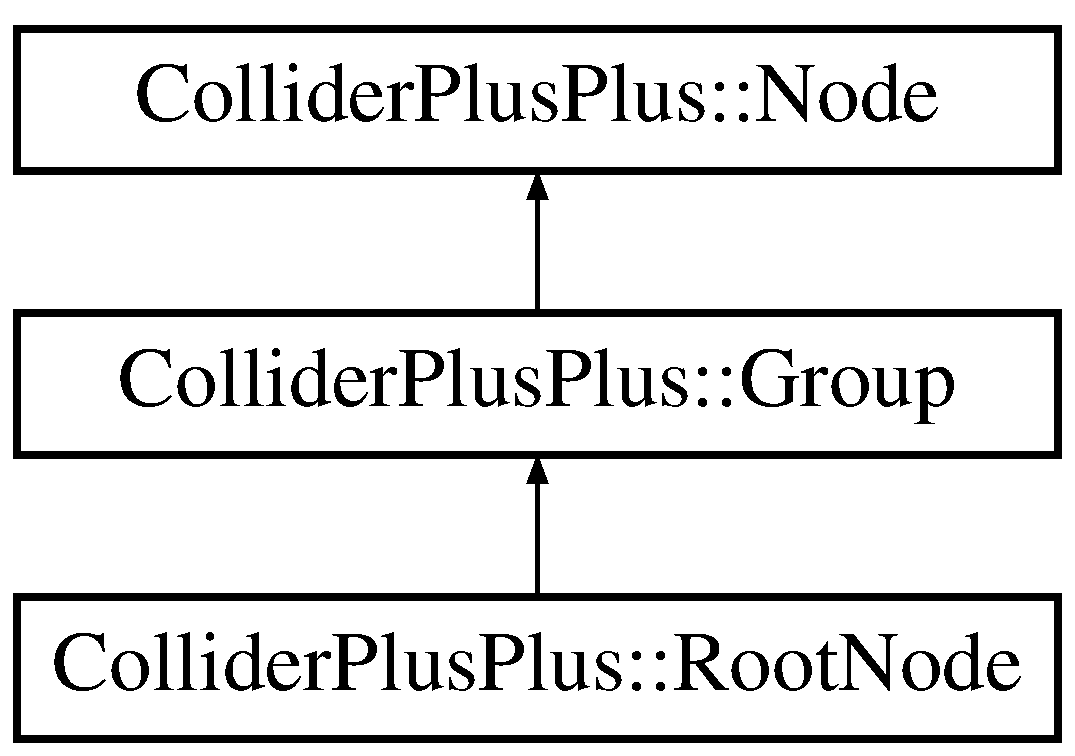
\includegraphics[height=3.000000cm]{classColliderPlusPlus_1_1Group}
\end{center}
\end{figure}
\subsection*{Public Member Functions}
\begin{DoxyCompactItemize}
\item 
\hyperlink{classColliderPlusPlus_1_1Group_aaacdebb53fcb4acabc16d4d7f780364a}{Group} (\hyperlink{classColliderPlusPlus_1_1Client__Server}{Client\-\_\-\-Server} \&cs, const std\-::string \&name, int id, int add\-Action=T\-O\-\_\-\-H\-E\-A\-D, int target=D\-E\-F\-A\-U\-L\-T\-\_\-\-G\-R\-O\-U\-P)
\item 
\hypertarget{classColliderPlusPlus_1_1Group_aa7f0bbd9db8735ee8dc5fdfc8c7239cf}{\hyperlink{classColliderPlusPlus_1_1Group_aa7f0bbd9db8735ee8dc5fdfc8c7239cf}{$\sim$\-Group} ()}\label{classColliderPlusPlus_1_1Group_aa7f0bbd9db8735ee8dc5fdfc8c7239cf}

\begin{DoxyCompactList}\small\item\em Destructor. \end{DoxyCompactList}\item 
void \hyperlink{classColliderPlusPlus_1_1Group_aff4f20b6099abba697333e079e7bbeb3}{\-\_\-free\-All\-Synths} (\hyperlink{classColliderPlusPlus_1_1Client__Server}{Client\-\_\-\-Server} \&cs)
\item 
void \hyperlink{classColliderPlusPlus_1_1Group_a843a985ffb36764b5e568560a2ea9608}{\-\_\-deep\-Free\-All\-Synths} (\hyperlink{classColliderPlusPlus_1_1Client__Server}{Client\-\_\-\-Server} \&cs)
\end{DoxyCompactItemize}
\subsection*{Additional Inherited Members}


\subsection{Detailed Description}
This class represents a client-\/side version of a server group. 

\subsection{Constructor \& Destructor Documentation}
\hypertarget{classColliderPlusPlus_1_1Group_aaacdebb53fcb4acabc16d4d7f780364a}{\index{Collider\-Plus\-Plus\-::\-Group@{Collider\-Plus\-Plus\-::\-Group}!Group@{Group}}
\index{Group@{Group}!ColliderPlusPlus::Group@{Collider\-Plus\-Plus\-::\-Group}}
\subsubsection[{Group}]{\setlength{\rightskip}{0pt plus 5cm}Collider\-Plus\-Plus\-::\-Group\-::\-Group (
\begin{DoxyParamCaption}
\item[{{\bf Client\-\_\-\-Server} \&}]{cs, }
\item[{const std\-::string \&}]{name, }
\item[{int}]{id, }
\item[{int}]{add\-Action = {\ttfamily TO\-\_\-HEAD}, }
\item[{int}]{target = {\ttfamily DEFAULT\-\_\-GROUP}}
\end{DoxyParamCaption}
)}}\label{classColliderPlusPlus_1_1Group_aaacdebb53fcb4acabc16d4d7f780364a}
Create a \hyperlink{classColliderPlusPlus_1_1Group}{Group} with a user defined name, id, add\-Action, and target If no add\-Action is specified, this \hyperlink{classColliderPlusPlus_1_1Group}{Group} is added to the head of target group If no target group is specified, this \hyperlink{classColliderPlusPlus_1_1Synth}{Synth} is added to the Default \hyperlink{classColliderPlusPlus_1_1Group}{Group} 
\begin{DoxyParams}[1]{Parameters}
\mbox{\tt in}  & {\em Client\-\_\-\-Server\&} & \hyperlink{classColliderPlusPlus_1_1Client__Server}{Client\-\_\-\-Server} instance \\
\hline
\mbox{\tt in}  & {\em const} & std\-::string\& Name \\
\hline
\mbox{\tt in}  & {\em int} & Id \\
\hline
\mbox{\tt in}  & {\em int} & Add Action \\
\hline
\mbox{\tt in}  & {\em int} & Target \hyperlink{classColliderPlusPlus_1_1Group}{Group} \\
\hline
\end{DoxyParams}


\subsection{Member Function Documentation}
\hypertarget{classColliderPlusPlus_1_1Group_a843a985ffb36764b5e568560a2ea9608}{\index{Collider\-Plus\-Plus\-::\-Group@{Collider\-Plus\-Plus\-::\-Group}!\-\_\-deep\-Free\-All\-Synths@{\-\_\-deep\-Free\-All\-Synths}}
\index{\-\_\-deep\-Free\-All\-Synths@{\-\_\-deep\-Free\-All\-Synths}!ColliderPlusPlus::Group@{Collider\-Plus\-Plus\-::\-Group}}
\subsubsection[{\-\_\-deep\-Free\-All\-Synths}]{\setlength{\rightskip}{0pt plus 5cm}void Collider\-Plus\-Plus\-::\-Group\-::\-\_\-deep\-Free\-All\-Synths (
\begin{DoxyParamCaption}
\item[{{\bf Client\-\_\-\-Server} \&}]{cs}
\end{DoxyParamCaption}
)}}\label{classColliderPlusPlus_1_1Group_a843a985ffb36764b5e568560a2ea9608}
Free all Nodes in this \hyperlink{classColliderPlusPlus_1_1Group}{Group} and in all Sub-\/\-Groups 
\begin{DoxyParams}[1]{Parameters}
\mbox{\tt in}  & {\em Client\-\_\-\-Server\&} & \hyperlink{classColliderPlusPlus_1_1Client__Server}{Client\-\_\-\-Server} instance \\
\hline
\end{DoxyParams}
\hypertarget{classColliderPlusPlus_1_1Group_aff4f20b6099abba697333e079e7bbeb3}{\index{Collider\-Plus\-Plus\-::\-Group@{Collider\-Plus\-Plus\-::\-Group}!\-\_\-free\-All\-Synths@{\-\_\-free\-All\-Synths}}
\index{\-\_\-free\-All\-Synths@{\-\_\-free\-All\-Synths}!ColliderPlusPlus::Group@{Collider\-Plus\-Plus\-::\-Group}}
\subsubsection[{\-\_\-free\-All\-Synths}]{\setlength{\rightskip}{0pt plus 5cm}void Collider\-Plus\-Plus\-::\-Group\-::\-\_\-free\-All\-Synths (
\begin{DoxyParamCaption}
\item[{{\bf Client\-\_\-\-Server} \&}]{cs}
\end{DoxyParamCaption}
)}}\label{classColliderPlusPlus_1_1Group_aff4f20b6099abba697333e079e7bbeb3}
Free all Nodes in this \hyperlink{classColliderPlusPlus_1_1Group}{Group} 
\begin{DoxyParams}[1]{Parameters}
\mbox{\tt in}  & {\em Client\-\_\-\-Server\&} & \hyperlink{classColliderPlusPlus_1_1Client__Server}{Client\-\_\-\-Server} instance \\
\hline
\end{DoxyParams}


The documentation for this class was generated from the following file\-:\begin{DoxyCompactItemize}
\item 
include/\hyperlink{Node_8hpp}{Node.\-hpp}\end{DoxyCompactItemize}

\hypertarget{classColliderPlusPlus_1_1Node}{\section{Collider\-Plus\-Plus\-:\-:Node Class Reference}
\label{classColliderPlusPlus_1_1Node}\index{Collider\-Plus\-Plus\-::\-Node@{Collider\-Plus\-Plus\-::\-Node}}
}


This class represents a client-\/side version of a server node (\hyperlink{classColliderPlusPlus_1_1Synth}{Synth} or \hyperlink{classColliderPlusPlus_1_1Group}{Group})  




{\ttfamily \#include $<$Node.\-hpp$>$}

Inheritance diagram for Collider\-Plus\-Plus\-:\-:Node\-:\begin{figure}[H]
\begin{center}
\leavevmode
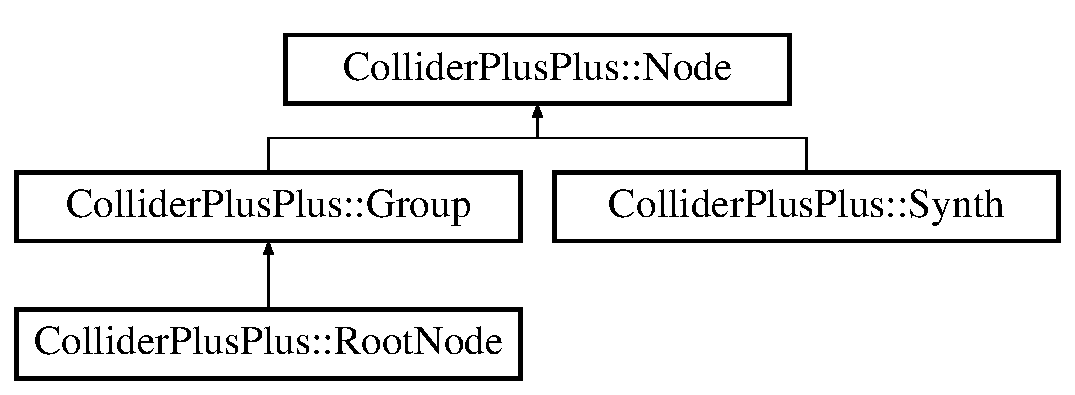
\includegraphics[height=3.000000cm]{classColliderPlusPlus_1_1Node}
\end{center}
\end{figure}
\subsection*{Public Member Functions}
\begin{DoxyCompactItemize}
\item 
\hypertarget{classColliderPlusPlus_1_1Node_aaad80bfe23840414c3522f5a25f5771a}{\hyperlink{classColliderPlusPlus_1_1Node_aaad80bfe23840414c3522f5a25f5771a}{Node} ()}\label{classColliderPlusPlus_1_1Node_aaad80bfe23840414c3522f5a25f5771a}

\begin{DoxyCompactList}\small\item\em Default Constructor. \end{DoxyCompactList}\item 
\hyperlink{classColliderPlusPlus_1_1Node_a306340cc9340b97bbdd0df858c8a4185}{Node} (const std\-::string \&def\-Name, int id)
\item 
\hypertarget{classColliderPlusPlus_1_1Node_ae1198291ae5d81dd34474b7cf52438cd}{\hyperlink{classColliderPlusPlus_1_1Node_ae1198291ae5d81dd34474b7cf52438cd}{$\sim$\-Node} ()}\label{classColliderPlusPlus_1_1Node_ae1198291ae5d81dd34474b7cf52438cd}

\begin{DoxyCompactList}\small\item\em Destructor. \end{DoxyCompactList}\item 
int \hyperlink{classColliderPlusPlus_1_1Node_a261794de64a2198ca94e2c6410f3845f}{\-\_\-get\-Id} () const 
\item 
\hypertarget{classColliderPlusPlus_1_1Node_a97a4981f950823a4326bd87caa7826f0}{void \hyperlink{classColliderPlusPlus_1_1Node_a97a4981f950823a4326bd87caa7826f0}{\-\_\-run} (\hyperlink{classColliderPlusPlus_1_1Client__Server}{Client\-\_\-\-Server} \&cs)}\label{classColliderPlusPlus_1_1Node_a97a4981f950823a4326bd87caa7826f0}

\begin{DoxyCompactList}\small\item\em Command the server to run this \hyperlink{classColliderPlusPlus_1_1Node}{Node}. \end{DoxyCompactList}\item 
\hypertarget{classColliderPlusPlus_1_1Node_acb5dda7d418dfb041871815f2828f1ba}{void \hyperlink{classColliderPlusPlus_1_1Node_acb5dda7d418dfb041871815f2828f1ba}{\-\_\-stop} (\hyperlink{classColliderPlusPlus_1_1Client__Server}{Client\-\_\-\-Server} \&cs)}\label{classColliderPlusPlus_1_1Node_acb5dda7d418dfb041871815f2828f1ba}

\begin{DoxyCompactList}\small\item\em Command the server to stop this \hyperlink{classColliderPlusPlus_1_1Node}{Node}. \end{DoxyCompactList}\item 
\hypertarget{classColliderPlusPlus_1_1Node_abca0b4c65fc62a5f749bc8c9d9898211}{void \hyperlink{classColliderPlusPlus_1_1Node_abca0b4c65fc62a5f749bc8c9d9898211}{\-\_\-free} (\hyperlink{classColliderPlusPlus_1_1Client__Server}{Client\-\_\-\-Server} \&cs)}\label{classColliderPlusPlus_1_1Node_abca0b4c65fc62a5f749bc8c9d9898211}

\begin{DoxyCompactList}\small\item\em Command the server to free this \hyperlink{classColliderPlusPlus_1_1Node}{Node}. \end{DoxyCompactList}\item 
bool \hyperlink{classColliderPlusPlus_1_1Node_a52123c9868b5e1833750158c870c3b87}{\-\_\-is\-Playing} ()
\item 
bool \hyperlink{classColliderPlusPlus_1_1Node_a5f073a198b55b4c471e772ca2661d144}{\-\_\-is\-Running} ()
\item 
std\-::string \hyperlink{classColliderPlusPlus_1_1Node_a47ab8ce687a4336189a6cc629cdec56d}{\-\_\-get\-Def\-Name} () const 
\item 
\hypertarget{classColliderPlusPlus_1_1Node_a796ea51c38b6894b93ebafe8eae316b9}{void \hyperlink{classColliderPlusPlus_1_1Node_a796ea51c38b6894b93ebafe8eae316b9}{\-\_\-query} (\hyperlink{classColliderPlusPlus_1_1Client__Server}{Client\-\_\-\-Server} \&cs)}\label{classColliderPlusPlus_1_1Node_a796ea51c38b6894b93ebafe8eae316b9}

\begin{DoxyCompactList}\small\item\em Query the server for this \hyperlink{classColliderPlusPlus_1_1Node}{Node}. \end{DoxyCompactList}\end{DoxyCompactItemize}
\begin{Indent}{\bf Control and Bus Mapping Functions}\par
\begin{DoxyCompactItemize}
\item 
void \hyperlink{classColliderPlusPlus_1_1Node_a114d15e7c1f14462983f602fb2164dc1}{\-\_\-set} (\hyperlink{classColliderPlusPlus_1_1Client__Server}{Client\-\_\-\-Server} \&cs, std\-::map$<$ std\-::string, float $>$ \&control\-Vals)
\item 
void \hyperlink{classColliderPlusPlus_1_1Node_aef01261b4c0d4046c63a857b864ae824}{\-\_\-setn} (\hyperlink{classColliderPlusPlus_1_1Client__Server}{Client\-\_\-\-Server} \&cs, std\-::map$<$ std\-::string, float\mbox{[}$\,$\mbox{]}$>$ \&control\-Ranges)
\item 
void \hyperlink{classColliderPlusPlus_1_1Node_af654f15c4f2de2b96b69c1992d6de33e}{\-\_\-bus\-Map} (\hyperlink{classColliderPlusPlus_1_1Client__Server}{Client\-\_\-\-Server} \&cs, std\-::map$<$ std\-::string, \hyperlink{classColliderPlusPlus_1_1Bus}{Bus} $>$ \&map)
\end{DoxyCompactItemize}
\end{Indent}
\subsection*{Protected Attributes}
\begin{DoxyCompactItemize}
\item 
\hypertarget{classColliderPlusPlus_1_1Node_a089f73464d3a7c0f9f7432a02779cafa}{int {\bfseries \-\_\-id}}\label{classColliderPlusPlus_1_1Node_a089f73464d3a7c0f9f7432a02779cafa}

\item 
\hypertarget{classColliderPlusPlus_1_1Node_ad37555cf7d7cbccf7dc564cf9fb519b3}{std\-::string {\bfseries \-\_\-def\-Name}}\label{classColliderPlusPlus_1_1Node_ad37555cf7d7cbccf7dc564cf9fb519b3}

\item 
\hypertarget{classColliderPlusPlus_1_1Node_a6e76eb59c93e21a54e6ce3c1635b107e}{bool {\bfseries \-\_\-playing}}\label{classColliderPlusPlus_1_1Node_a6e76eb59c93e21a54e6ce3c1635b107e}

\item 
\hypertarget{classColliderPlusPlus_1_1Node_af8d1c6e6e3997fd110158816282490a9}{bool {\bfseries \-\_\-running}}\label{classColliderPlusPlus_1_1Node_af8d1c6e6e3997fd110158816282490a9}

\end{DoxyCompactItemize}


\subsection{Detailed Description}
This class represents a client-\/side version of a server node (\hyperlink{classColliderPlusPlus_1_1Synth}{Synth} or \hyperlink{classColliderPlusPlus_1_1Group}{Group}) 

\subsection{Constructor \& Destructor Documentation}
\hypertarget{classColliderPlusPlus_1_1Node_a306340cc9340b97bbdd0df858c8a4185}{\index{Collider\-Plus\-Plus\-::\-Node@{Collider\-Plus\-Plus\-::\-Node}!Node@{Node}}
\index{Node@{Node}!ColliderPlusPlus::Node@{Collider\-Plus\-Plus\-::\-Node}}
\subsubsection[{Node}]{\setlength{\rightskip}{0pt plus 5cm}Collider\-Plus\-Plus\-::\-Node\-::\-Node (
\begin{DoxyParamCaption}
\item[{const std\-::string \&}]{def\-Name, }
\item[{int}]{id}
\end{DoxyParamCaption}
)}}\label{classColliderPlusPlus_1_1Node_a306340cc9340b97bbdd0df858c8a4185}
Create a \hyperlink{classColliderPlusPlus_1_1Node}{Node} with a user defined name and Id 
\begin{DoxyParams}[1]{Parameters}
\mbox{\tt in}  & {\em const} & std\-::string\& Name \\
\hline
\mbox{\tt in}  & {\em int} & Id \\
\hline
\end{DoxyParams}


\subsection{Member Function Documentation}
\hypertarget{classColliderPlusPlus_1_1Node_af654f15c4f2de2b96b69c1992d6de33e}{\index{Collider\-Plus\-Plus\-::\-Node@{Collider\-Plus\-Plus\-::\-Node}!\-\_\-bus\-Map@{\-\_\-bus\-Map}}
\index{\-\_\-bus\-Map@{\-\_\-bus\-Map}!ColliderPlusPlus::Node@{Collider\-Plus\-Plus\-::\-Node}}
\subsubsection[{\-\_\-bus\-Map}]{\setlength{\rightskip}{0pt plus 5cm}void Collider\-Plus\-Plus\-::\-Node\-::\-\_\-bus\-Map (
\begin{DoxyParamCaption}
\item[{{\bf Client\-\_\-\-Server} \&}]{cs, }
\item[{std\-::map$<$ std\-::string, {\bf Bus} $>$ \&}]{map}
\end{DoxyParamCaption}
)}}\label{classColliderPlusPlus_1_1Node_af654f15c4f2de2b96b69c1992d6de33e}
Set this \hyperlink{classColliderPlusPlus_1_1Node}{Node} with specified bus mappings 
\begin{DoxyParams}[1]{Parameters}
\mbox{\tt in}  & {\em Client\-\_\-\-Server\&} & \hyperlink{classColliderPlusPlus_1_1Client__Server}{Client\-\_\-\-Server} instance \\
\hline
\mbox{\tt in}  & {\em std\-::map$<$std\-::string,Bus$>$\&} & map \\
\hline
\end{DoxyParams}
\hypertarget{classColliderPlusPlus_1_1Node_a47ab8ce687a4336189a6cc629cdec56d}{\index{Collider\-Plus\-Plus\-::\-Node@{Collider\-Plus\-Plus\-::\-Node}!\-\_\-get\-Def\-Name@{\-\_\-get\-Def\-Name}}
\index{\-\_\-get\-Def\-Name@{\-\_\-get\-Def\-Name}!ColliderPlusPlus::Node@{Collider\-Plus\-Plus\-::\-Node}}
\subsubsection[{\-\_\-get\-Def\-Name}]{\setlength{\rightskip}{0pt plus 5cm}std\-::string Collider\-Plus\-Plus\-::\-Node\-::\-\_\-get\-Def\-Name (
\begin{DoxyParamCaption}
{}
\end{DoxyParamCaption}
) const\hspace{0.3cm}{\ttfamily [inline]}}}\label{classColliderPlusPlus_1_1Node_a47ab8ce687a4336189a6cc629cdec56d}
Returns the name of this \hyperlink{classColliderPlusPlus_1_1Node}{Node} \begin{DoxyReturn}{Returns}
\-\_\-def\-Name 
\end{DoxyReturn}
\hypertarget{classColliderPlusPlus_1_1Node_a261794de64a2198ca94e2c6410f3845f}{\index{Collider\-Plus\-Plus\-::\-Node@{Collider\-Plus\-Plus\-::\-Node}!\-\_\-get\-Id@{\-\_\-get\-Id}}
\index{\-\_\-get\-Id@{\-\_\-get\-Id}!ColliderPlusPlus::Node@{Collider\-Plus\-Plus\-::\-Node}}
\subsubsection[{\-\_\-get\-Id}]{\setlength{\rightskip}{0pt plus 5cm}int Collider\-Plus\-Plus\-::\-Node\-::\-\_\-get\-Id (
\begin{DoxyParamCaption}
{}
\end{DoxyParamCaption}
) const\hspace{0.3cm}{\ttfamily [inline]}}}\label{classColliderPlusPlus_1_1Node_a261794de64a2198ca94e2c6410f3845f}
Returns the Id of this \hyperlink{classColliderPlusPlus_1_1Node}{Node} \begin{DoxyReturn}{Returns}
\-\_\-id 
\end{DoxyReturn}
\hypertarget{classColliderPlusPlus_1_1Node_a52123c9868b5e1833750158c870c3b87}{\index{Collider\-Plus\-Plus\-::\-Node@{Collider\-Plus\-Plus\-::\-Node}!\-\_\-is\-Playing@{\-\_\-is\-Playing}}
\index{\-\_\-is\-Playing@{\-\_\-is\-Playing}!ColliderPlusPlus::Node@{Collider\-Plus\-Plus\-::\-Node}}
\subsubsection[{\-\_\-is\-Playing}]{\setlength{\rightskip}{0pt plus 5cm}bool Collider\-Plus\-Plus\-::\-Node\-::\-\_\-is\-Playing (
\begin{DoxyParamCaption}
{}
\end{DoxyParamCaption}
)\hspace{0.3cm}{\ttfamily [inline]}}}\label{classColliderPlusPlus_1_1Node_a52123c9868b5e1833750158c870c3b87}
Returns true if this \hyperlink{classColliderPlusPlus_1_1Node}{Node} is currently playing, else false \begin{DoxyReturn}{Returns}
true if currently playing, else false 
\end{DoxyReturn}
\hypertarget{classColliderPlusPlus_1_1Node_a5f073a198b55b4c471e772ca2661d144}{\index{Collider\-Plus\-Plus\-::\-Node@{Collider\-Plus\-Plus\-::\-Node}!\-\_\-is\-Running@{\-\_\-is\-Running}}
\index{\-\_\-is\-Running@{\-\_\-is\-Running}!ColliderPlusPlus::Node@{Collider\-Plus\-Plus\-::\-Node}}
\subsubsection[{\-\_\-is\-Running}]{\setlength{\rightskip}{0pt plus 5cm}bool Collider\-Plus\-Plus\-::\-Node\-::\-\_\-is\-Running (
\begin{DoxyParamCaption}
{}
\end{DoxyParamCaption}
)\hspace{0.3cm}{\ttfamily [inline]}}}\label{classColliderPlusPlus_1_1Node_a5f073a198b55b4c471e772ca2661d144}
Returns true if this \hyperlink{classColliderPlusPlus_1_1Node}{Node} is currently running, else false \begin{DoxyReturn}{Returns}
true if currently running, else false 
\end{DoxyReturn}
\hypertarget{classColliderPlusPlus_1_1Node_a114d15e7c1f14462983f602fb2164dc1}{\index{Collider\-Plus\-Plus\-::\-Node@{Collider\-Plus\-Plus\-::\-Node}!\-\_\-set@{\-\_\-set}}
\index{\-\_\-set@{\-\_\-set}!ColliderPlusPlus::Node@{Collider\-Plus\-Plus\-::\-Node}}
\subsubsection[{\-\_\-set}]{\setlength{\rightskip}{0pt plus 5cm}void Collider\-Plus\-Plus\-::\-Node\-::\-\_\-set (
\begin{DoxyParamCaption}
\item[{{\bf Client\-\_\-\-Server} \&}]{cs, }
\item[{std\-::map$<$ std\-::string, float $>$ \&}]{control\-Vals}
\end{DoxyParamCaption}
)}}\label{classColliderPlusPlus_1_1Node_a114d15e7c1f14462983f602fb2164dc1}
Set this \hyperlink{classColliderPlusPlus_1_1Node}{Node} with specified control values 
\begin{DoxyParams}[1]{Parameters}
\mbox{\tt in}  & {\em Client\-\_\-\-Server\&} & \hyperlink{classColliderPlusPlus_1_1Client__Server}{Client\-\_\-\-Server} instance \\
\hline
\mbox{\tt in}  & {\em std\-::map$<$std\-::string,float$>$\&} & Control Values \\
\hline
\end{DoxyParams}
\hypertarget{classColliderPlusPlus_1_1Node_aef01261b4c0d4046c63a857b864ae824}{\index{Collider\-Plus\-Plus\-::\-Node@{Collider\-Plus\-Plus\-::\-Node}!\-\_\-setn@{\-\_\-setn}}
\index{\-\_\-setn@{\-\_\-setn}!ColliderPlusPlus::Node@{Collider\-Plus\-Plus\-::\-Node}}
\subsubsection[{\-\_\-setn}]{\setlength{\rightskip}{0pt plus 5cm}void Collider\-Plus\-Plus\-::\-Node\-::\-\_\-setn (
\begin{DoxyParamCaption}
\item[{{\bf Client\-\_\-\-Server} \&}]{cs, }
\item[{std\-::map$<$ std\-::string, float\mbox{[}$\,$\mbox{]}$>$ \&}]{control\-Ranges}
\end{DoxyParamCaption}
)}}\label{classColliderPlusPlus_1_1Node_aef01261b4c0d4046c63a857b864ae824}
Set this \hyperlink{classColliderPlusPlus_1_1Node}{Node} with specified control range values 
\begin{DoxyParams}[1]{Parameters}
\mbox{\tt in}  & {\em Client\-\_\-\-Server\&} & \hyperlink{classColliderPlusPlus_1_1Client__Server}{Client\-\_\-\-Server} instance \\
\hline
\mbox{\tt in}  & {\em std\-::map$<$std\-::string,float\mbox{[}$\,$\mbox{]}$>$\&} & Control Ranges \\
\hline
\end{DoxyParams}


The documentation for this class was generated from the following file\-:\begin{DoxyCompactItemize}
\item 
include/\hyperlink{Node_8hpp}{Node.\-hpp}\end{DoxyCompactItemize}

\hypertarget{classColliderPlusPlus_1_1RootNode}{\section{Collider\-Plus\-Plus\-:\-:Root\-Node Class Reference}
\label{classColliderPlusPlus_1_1RootNode}\index{Collider\-Plus\-Plus\-::\-Root\-Node@{Collider\-Plus\-Plus\-::\-Root\-Node}}
}


This class represents a client-\/side version of a server root node.  




{\ttfamily \#include $<$Node.\-hpp$>$}

Inheritance diagram for Collider\-Plus\-Plus\-:\-:Root\-Node\-:\begin{figure}[H]
\begin{center}
\leavevmode
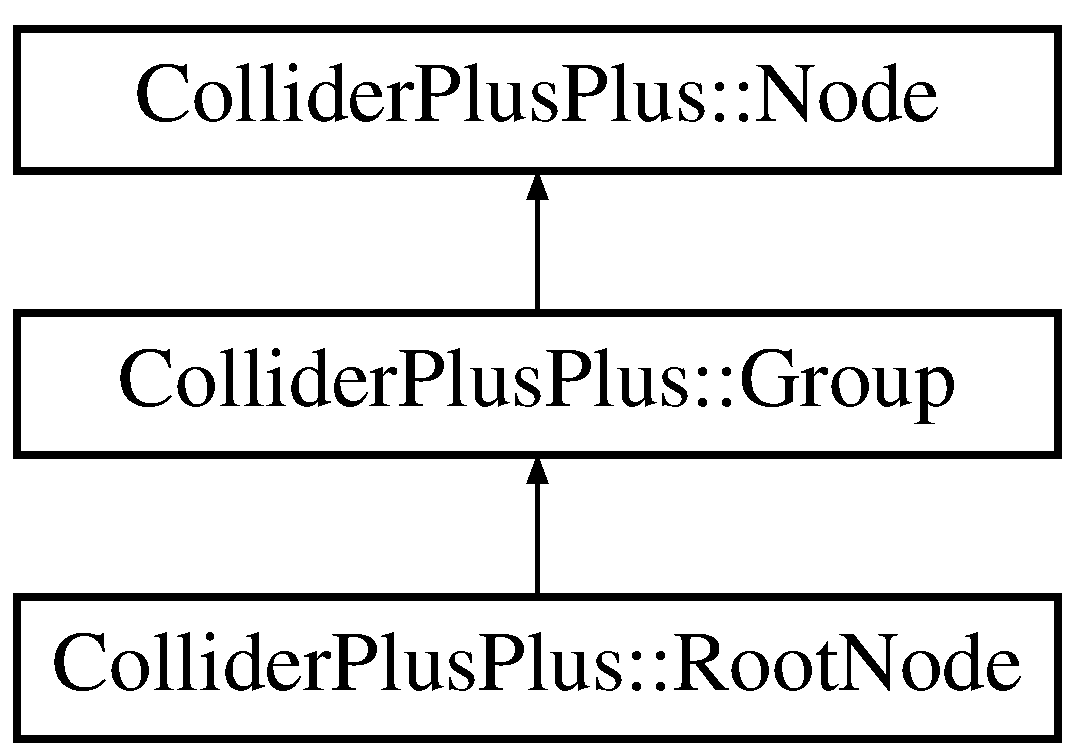
\includegraphics[height=3.000000cm]{classColliderPlusPlus_1_1RootNode}
\end{center}
\end{figure}
\subsection*{Public Member Functions}
\begin{DoxyCompactItemize}
\item 
\hyperlink{classColliderPlusPlus_1_1RootNode_ab1a4476f355e19055fa056802e7ffee9}{Root\-Node} (\hyperlink{classColliderPlusPlus_1_1Client__Server}{Client\-\_\-\-Server} \&cs)
\item 
\hypertarget{classColliderPlusPlus_1_1RootNode_ae8b5552c4652ee2a5b9079124a1b7a76}{\hyperlink{classColliderPlusPlus_1_1RootNode_ae8b5552c4652ee2a5b9079124a1b7a76}{$\sim$\-Root\-Node} ()}\label{classColliderPlusPlus_1_1RootNode_ae8b5552c4652ee2a5b9079124a1b7a76}

\begin{DoxyCompactList}\small\item\em Destructor. \end{DoxyCompactList}\end{DoxyCompactItemize}
\subsection*{Additional Inherited Members}


\subsection{Detailed Description}
This class represents a client-\/side version of a server root node. 

\subsection{Constructor \& Destructor Documentation}
\hypertarget{classColliderPlusPlus_1_1RootNode_ab1a4476f355e19055fa056802e7ffee9}{\index{Collider\-Plus\-Plus\-::\-Root\-Node@{Collider\-Plus\-Plus\-::\-Root\-Node}!Root\-Node@{Root\-Node}}
\index{Root\-Node@{Root\-Node}!ColliderPlusPlus::RootNode@{Collider\-Plus\-Plus\-::\-Root\-Node}}
\subsubsection[{Root\-Node}]{\setlength{\rightskip}{0pt plus 5cm}Root\-Node\-::\-Root\-Node (
\begin{DoxyParamCaption}
\item[{{\bf Client\-\_\-\-Server} \&}]{cs}
\end{DoxyParamCaption}
)}}\label{classColliderPlusPlus_1_1RootNode_ab1a4476f355e19055fa056802e7ffee9}
Create a Root \hyperlink{classColliderPlusPlus_1_1Node}{Node} 
\begin{DoxyParams}[1]{Parameters}
\mbox{\tt in}  & {\em Client\-\_\-\-Server\&} & \hyperlink{classColliderPlusPlus_1_1Client__Server}{Client\-\_\-\-Server} instance \\
\hline
\end{DoxyParams}


The documentation for this class was generated from the following files\-:\begin{DoxyCompactItemize}
\item 
include/\hyperlink{Node_8hpp}{Node.\-hpp}\item 
src/Node.\-cpp\end{DoxyCompactItemize}

\hypertarget{classColliderPlusPlus_1_1Sound}{\section{Collider\-Plus\-Plus\-:\-:Sound Class Reference}
\label{classColliderPlusPlus_1_1Sound}\index{Collider\-Plus\-Plus\-::\-Sound@{Collider\-Plus\-Plus\-::\-Sound}}
}


This class represents a user manipulable Soundfile Player, essentially mirroring the O\-A\-S class of the same name by Shreenidhi Chowkwale  \href{https://github.com/CalVR/Open-Audio-Server/blob/master/client/src/Sound.h}{\tt https\-://github.\-com/\-Cal\-V\-R/\-Open-\/\-Audio-\/\-Server/blob/master/client/src/\-Sound.\-h}.  




{\ttfamily \#include $<$Sound.\-hpp$>$}

\subsection*{Public Member Functions}
\begin{DoxyCompactItemize}
\item 
\hypertarget{classColliderPlusPlus_1_1Sound_ac1e87781b6bb69d6a250d2eaab360994}{\hyperlink{classColliderPlusPlus_1_1Sound_ac1e87781b6bb69d6a250d2eaab360994}{Sound} (\hyperlink{classColliderPlusPlus_1_1Client__Server}{Client\-\_\-\-Server} $\ast$other, const std\-::string \&filepath, int init\-Action=0)}\label{classColliderPlusPlus_1_1Sound_ac1e87781b6bb69d6a250d2eaab360994}

\begin{DoxyCompactList}\small\item\em Create a new sound source. \end{DoxyCompactList}\item 
\hypertarget{classColliderPlusPlus_1_1Sound_a0ae9f80837e343e016952def28815072}{\hyperlink{classColliderPlusPlus_1_1Sound_a0ae9f80837e343e016952def28815072}{$\sim$\-Sound} ()}\label{classColliderPlusPlus_1_1Sound_a0ae9f80837e343e016952def28815072}

\begin{DoxyCompactList}\small\item\em Deallocates server-\/side buffer associated with this instance. \end{DoxyCompactList}\end{DoxyCompactItemize}
\begin{Indent}{\bf Playback Functions}\par
\begin{DoxyCompactItemize}
\item 
\hypertarget{classColliderPlusPlus_1_1Sound_a555d34089f5c74363b837ffaf4a66c45}{void \hyperlink{classColliderPlusPlus_1_1Sound_a555d34089f5c74363b837ffaf4a66c45}{play} ()}\label{classColliderPlusPlus_1_1Sound_a555d34089f5c74363b837ffaf4a66c45}

\begin{DoxyCompactList}\small\item\em Play the sound source from the last position. \end{DoxyCompactList}\item 
\hypertarget{classColliderPlusPlus_1_1Sound_a7010e6bcdd47d51b359c364883574a5d}{void \hyperlink{classColliderPlusPlus_1_1Sound_a7010e6bcdd47d51b359c364883574a5d}{stop} ()}\label{classColliderPlusPlus_1_1Sound_a7010e6bcdd47d51b359c364883574a5d}

\begin{DoxyCompactList}\small\item\em Pauses the sound source at the current playback position. \end{DoxyCompactList}\item 
int \hyperlink{classColliderPlusPlus_1_1Sound_aad17d4b990faae4cf90c281e33d06155}{loop} (bool loop)
\end{DoxyCompactItemize}
\end{Indent}
\begin{Indent}{\bf Sound Parameter Functions}\par
\begin{DoxyCompactItemize}
\item 
void \hyperlink{classColliderPlusPlus_1_1Sound_ab64f46659f59a6d7b7bc206cca6402cf}{set\-Gain} (float gain)
\item 
void \hyperlink{classColliderPlusPlus_1_1Sound_a5bd234602a61929747697677d972fc30}{set\-Rate} (float rate\-Scalar)
\end{DoxyCompactItemize}
\end{Indent}


\subsection{Detailed Description}
This class represents a user manipulable Soundfile Player, essentially mirroring the O\-A\-S class of the same name by Shreenidhi Chowkwale  \href{https://github.com/CalVR/Open-Audio-Server/blob/master/client/src/Sound.h}{\tt https\-://github.\-com/\-Cal\-V\-R/\-Open-\/\-Audio-\/\-Server/blob/master/client/src/\-Sound.\-h}. 

\subsection{Member Function Documentation}
\hypertarget{classColliderPlusPlus_1_1Sound_aad17d4b990faae4cf90c281e33d06155}{\index{Collider\-Plus\-Plus\-::\-Sound@{Collider\-Plus\-Plus\-::\-Sound}!loop@{loop}}
\index{loop@{loop}!ColliderPlusPlus::Sound@{Collider\-Plus\-Plus\-::\-Sound}}
\subsubsection[{loop}]{\setlength{\rightskip}{0pt plus 5cm}int Collider\-Plus\-Plus\-::\-Sound\-::loop (
\begin{DoxyParamCaption}
\item[{bool}]{loop}
\end{DoxyParamCaption}
)}}\label{classColliderPlusPlus_1_1Sound_aad17d4b990faae4cf90c281e33d06155}
Set the looping state false = no looping, true = looping 
\begin{DoxyParams}[1]{Parameters}
\mbox{\tt in}  & {\em bool} & loop \\
\hline
\end{DoxyParams}
\hypertarget{classColliderPlusPlus_1_1Sound_ab64f46659f59a6d7b7bc206cca6402cf}{\index{Collider\-Plus\-Plus\-::\-Sound@{Collider\-Plus\-Plus\-::\-Sound}!set\-Gain@{set\-Gain}}
\index{set\-Gain@{set\-Gain}!ColliderPlusPlus::Sound@{Collider\-Plus\-Plus\-::\-Sound}}
\subsubsection[{set\-Gain}]{\setlength{\rightskip}{0pt plus 5cm}void Collider\-Plus\-Plus\-::\-Sound\-::set\-Gain (
\begin{DoxyParamCaption}
\item[{float}]{gain}
\end{DoxyParamCaption}
)}}\label{classColliderPlusPlus_1_1Sound_ab64f46659f59a6d7b7bc206cca6402cf}
Set the current gain from 0 -\/ 1 
\begin{DoxyParams}[1]{Parameters}
\mbox{\tt in}  & {\em float} & gain \\
\hline
\end{DoxyParams}
\hypertarget{classColliderPlusPlus_1_1Sound_a5bd234602a61929747697677d972fc30}{\index{Collider\-Plus\-Plus\-::\-Sound@{Collider\-Plus\-Plus\-::\-Sound}!set\-Rate@{set\-Rate}}
\index{set\-Rate@{set\-Rate}!ColliderPlusPlus::Sound@{Collider\-Plus\-Plus\-::\-Sound}}
\subsubsection[{set\-Rate}]{\setlength{\rightskip}{0pt plus 5cm}void Collider\-Plus\-Plus\-::\-Sound\-::set\-Rate (
\begin{DoxyParamCaption}
\item[{float}]{rate\-Scalar}
\end{DoxyParamCaption}
)}}\label{classColliderPlusPlus_1_1Sound_a5bd234602a61929747697677d972fc30}
Set the current playback rate 1 is regular, 2 is double speed, .5 half speed etc. 
\begin{DoxyParams}[1]{Parameters}
\mbox{\tt in}  & {\em float} & rate\-Scalar \\
\hline
\end{DoxyParams}


The documentation for this class was generated from the following file\-:\begin{DoxyCompactItemize}
\item 
include/\hyperlink{Sound_8hpp}{Sound.\-hpp}\end{DoxyCompactItemize}

\hypertarget{classColliderPlusPlus_1_1Synth}{\section{Collider\-Plus\-Plus\-:\-:Synth Class Reference}
\label{classColliderPlusPlus_1_1Synth}\index{Collider\-Plus\-Plus\-::\-Synth@{Collider\-Plus\-Plus\-::\-Synth}}
}


This class represents a client-\/side version of a server synth.  




{\ttfamily \#include $<$Node.\-hpp$>$}

Inheritance diagram for Collider\-Plus\-Plus\-:\-:Synth\-:\begin{figure}[H]
\begin{center}
\leavevmode
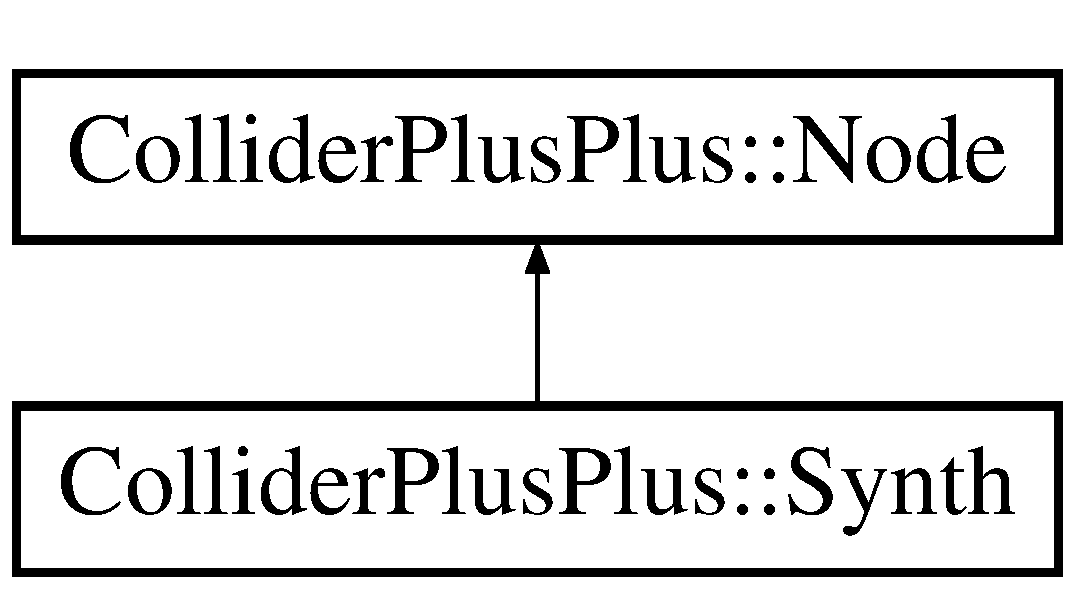
\includegraphics[height=2.000000cm]{classColliderPlusPlus_1_1Synth}
\end{center}
\end{figure}
\subsection*{Public Member Functions}
\begin{DoxyCompactItemize}
\item 
\hyperlink{classColliderPlusPlus_1_1Synth_a95d3df49d21a4c6844089ae7641a1be4}{Synth} (\hyperlink{classColliderPlusPlus_1_1Client__Server}{Client\-\_\-\-Server} $\ast$other, const std\-::string \&def\-Name, int id\-\_\-, int init\-Action=0, int add\-Action=T\-O\-\_\-\-H\-E\-A\-D, int target=D\-E\-F\-A\-U\-L\-T\-\_\-\-G\-R\-O\-U\-P)
\item 
\hyperlink{classColliderPlusPlus_1_1Synth_a6b1104ec5673c05ebe9d7804a1d85af8}{Synth} (\hyperlink{classColliderPlusPlus_1_1Client__Server}{Client\-\_\-\-Server} $\ast$other, const std\-::string \&def\-Name, int id\-\_\-, std\-::map$<$ std\-::string, float $>$ \&args, int init\-Action=0, int add\-Action=T\-O\-\_\-\-H\-E\-A\-D, int target=D\-E\-F\-A\-U\-L\-T\-\_\-\-G\-R\-O\-U\-P)
\item 
\hypertarget{classColliderPlusPlus_1_1Synth_a1fb61bf548db414b4dc543eac83216ae}{\hyperlink{classColliderPlusPlus_1_1Synth_a1fb61bf548db414b4dc543eac83216ae}{$\sim$\-Synth} ()}\label{classColliderPlusPlus_1_1Synth_a1fb61bf548db414b4dc543eac83216ae}

\begin{DoxyCompactList}\small\item\em Destructor. \end{DoxyCompactList}\end{DoxyCompactItemize}


\subsection{Detailed Description}
This class represents a client-\/side version of a server synth. 

\subsection{Constructor \& Destructor Documentation}
\hypertarget{classColliderPlusPlus_1_1Synth_a95d3df49d21a4c6844089ae7641a1be4}{\index{Collider\-Plus\-Plus\-::\-Synth@{Collider\-Plus\-Plus\-::\-Synth}!Synth@{Synth}}
\index{Synth@{Synth}!ColliderPlusPlus::Synth@{Collider\-Plus\-Plus\-::\-Synth}}
\subsubsection[{Synth}]{\setlength{\rightskip}{0pt plus 5cm}Collider\-Plus\-Plus\-::\-Synth\-::\-Synth (
\begin{DoxyParamCaption}
\item[{{\bf Client\-\_\-\-Server} $\ast$}]{other, }
\item[{const std\-::string \&}]{def\-Name, }
\item[{int}]{id\-\_\-, }
\item[{int}]{init\-Action = {\ttfamily 0}, }
\item[{int}]{add\-Action = {\ttfamily TO\-\_\-HEAD}, }
\item[{int}]{target = {\ttfamily DEFAULT\-\_\-GROUP}}
\end{DoxyParamCaption}
)}}\label{classColliderPlusPlus_1_1Synth_a95d3df49d21a4c6844089ae7641a1be4}
Create a \hyperlink{classColliderPlusPlus_1_1Synth}{Synth} with a user defined name, id, add\-Action, and target If no add\-Action is specified, this \hyperlink{classColliderPlusPlus_1_1Synth}{Synth} is added to the head of target group If no target group is specified, this \hyperlink{classColliderPlusPlus_1_1Synth}{Synth} is added to the Default \hyperlink{classColliderPlusPlus_1_1Group}{Group} 
\begin{DoxyParams}[1]{Parameters}
\mbox{\tt in}  & {\em Client\-\_\-\-Server\&} & \hyperlink{classColliderPlusPlus_1_1Client__Server}{Client\-\_\-\-Server} instance \\
\hline
\mbox{\tt in}  & {\em const} & std\-::string\& def\-Name \\
\hline
\mbox{\tt in}  & {\em int} & Id \\
\hline
\mbox{\tt in}  & {\em int} & Add Action \\
\hline
\mbox{\tt in}  & {\em int} & Target \hyperlink{classColliderPlusPlus_1_1Group}{Group} \\
\hline
\end{DoxyParams}
\hypertarget{classColliderPlusPlus_1_1Synth_a6b1104ec5673c05ebe9d7804a1d85af8}{\index{Collider\-Plus\-Plus\-::\-Synth@{Collider\-Plus\-Plus\-::\-Synth}!Synth@{Synth}}
\index{Synth@{Synth}!ColliderPlusPlus::Synth@{Collider\-Plus\-Plus\-::\-Synth}}
\subsubsection[{Synth}]{\setlength{\rightskip}{0pt plus 5cm}Collider\-Plus\-Plus\-::\-Synth\-::\-Synth (
\begin{DoxyParamCaption}
\item[{{\bf Client\-\_\-\-Server} $\ast$}]{other, }
\item[{const std\-::string \&}]{def\-Name, }
\item[{int}]{id\-\_\-, }
\item[{std\-::map$<$ std\-::string, float $>$ \&}]{args, }
\item[{int}]{init\-Action = {\ttfamily 0}, }
\item[{int}]{add\-Action = {\ttfamily TO\-\_\-HEAD}, }
\item[{int}]{target = {\ttfamily DEFAULT\-\_\-GROUP}}
\end{DoxyParamCaption}
)}}\label{classColliderPlusPlus_1_1Synth_a6b1104ec5673c05ebe9d7804a1d85af8}
Create a \hyperlink{classColliderPlusPlus_1_1Synth}{Synth} with a user defined name, id, \hyperlink{classColliderPlusPlus_1_1Node}{Node} args, add\-Action, and target If no add\-Action is specified, this \hyperlink{classColliderPlusPlus_1_1Synth}{Synth} is added to the head of target group If no target group is specified, this \hyperlink{classColliderPlusPlus_1_1Synth}{Synth} is added to the Default \hyperlink{classColliderPlusPlus_1_1Group}{Group} 
\begin{DoxyParams}[1]{Parameters}
\mbox{\tt in}  & {\em Client\-\_\-\-Server\&} & \hyperlink{classColliderPlusPlus_1_1Client__Server}{Client\-\_\-\-Server} instance \\
\hline
\mbox{\tt in}  & {\em const} & std\-::string\& def\-Name \\
\hline
\mbox{\tt in}  & {\em int} & Id \\
\hline
\mbox{\tt in}  & {\em std\-::map$<$std\-::string,float$>$} & Args \\
\hline
\mbox{\tt in}  & {\em int} & Add Action \\
\hline
\mbox{\tt in}  & {\em int} & Target \hyperlink{classColliderPlusPlus_1_1Group}{Group} \\
\hline
\end{DoxyParams}


The documentation for this class was generated from the following file\-:\begin{DoxyCompactItemize}
\item 
include/\hyperlink{Node_8hpp}{Node.\-hpp}\end{DoxyCompactItemize}

\chapter{File Documentation}
\hypertarget{Buffer_8hpp}{\section{include/\-Buffer.hpp File Reference}
\label{Buffer_8hpp}\index{include/\-Buffer.\-hpp@{include/\-Buffer.\-hpp}}
}


Header file for \hyperlink{Buffer_8hpp}{Buffer.\-hpp}.  


{\ttfamily \#include \char`\"{}S\-C\-Server.\-hpp\char`\"{}}\\*
\subsection*{Classes}
\begin{DoxyCompactItemize}
\item 
class \hyperlink{classsc_1_1Buffer}{sc\-::\-Buffer}
\begin{DoxyCompactList}\small\item\em This class represents a client-\/side version of a server buffer. \end{DoxyCompactList}\end{DoxyCompactItemize}


\subsection{Detailed Description}
Header file for \hyperlink{Buffer_8hpp}{Buffer.\-hpp}. \begin{DoxyAuthor}{Author}
Eric Hamdan \href{mailto:erichamdan@gmail.com}{\tt erichamdan@gmail.\-com} 
\end{DoxyAuthor}

\hypertarget{Bus_8hpp}{\section{include/\-Bus.hpp File Reference}
\label{Bus_8hpp}\index{include/\-Bus.\-hpp@{include/\-Bus.\-hpp}}
}


Header file for \hyperlink{Bus_8hpp}{Bus.\-hpp}.  


{\ttfamily \#include $<$vector$>$}\\*
\subsection*{Classes}
\begin{DoxyCompactItemize}
\item 
class \hyperlink{classColliderPlusPlus_1_1Bus}{Collider\-Plus\-Plus\-::\-Bus}
\begin{DoxyCompactList}\small\item\em This class represents a client-\/side version of a server bus. \end{DoxyCompactList}\end{DoxyCompactItemize}


\subsection{Detailed Description}
Header file for \hyperlink{Bus_8hpp}{Bus.\-hpp}. \begin{DoxyAuthor}{Author}
Eric Hamdan \href{mailto:erichamdan@gmail.com}{\tt erichamdan@gmail.\-com} 
\end{DoxyAuthor}

\hypertarget{Client__Server_8hpp}{\section{include/\-Client\-\_\-\-Server.hpp File Reference}
\label{Client__Server_8hpp}\index{include/\-Client\-\_\-\-Server.\-hpp@{include/\-Client\-\_\-\-Server.\-hpp}}
}


Header file for \hyperlink{Client__Server_8hpp}{Client\-\_\-\-Server.\-hpp}.  


{\ttfamily \#include $<$string$>$}\\*
{\ttfamily \#include $<$vector$>$}\\*
{\ttfamily \#include $<$map$>$}\\*
{\ttfamily \#include \char`\"{}tny\-\_\-osc/tnyosc-\/dispatch.\-hpp\char`\"{}}\\*
{\ttfamily \#include \char`\"{}tny\-\_\-osc/tnyosc.\-hpp\char`\"{}}\\*
\subsection*{Classes}
\begin{DoxyCompactItemize}
\item 
class \hyperlink{classColliderPlusPlus_1_1Client__Server}{Collider\-Plus\-Plus\-::\-Client\-\_\-\-Server}
\begin{DoxyCompactList}\small\item\em This class represents a client-\/side version of scsynth, the Super\-Collider audio server. \end{DoxyCompactList}\end{DoxyCompactItemize}
\subsection*{Macros}
\begin{DoxyCompactItemize}
\item 
\hypertarget{Client__Server_8hpp_aec2817847ec8c92eb99257101ddf102d}{\#define {\bfseries T\-O\-\_\-\-H\-E\-A\-D}~0}\label{Client__Server_8hpp_aec2817847ec8c92eb99257101ddf102d}

\item 
\hypertarget{Client__Server_8hpp_a1347de071d12a2e8a25f51b2cc7d6808}{\#define {\bfseries T\-O\-\_\-\-T\-A\-I\-L}~1}\label{Client__Server_8hpp_a1347de071d12a2e8a25f51b2cc7d6808}

\item 
\hypertarget{Client__Server_8hpp_a59b85f0c6cd4fecb4b22fc304b3f987b}{\#define {\bfseries J\-U\-S\-T\-\_\-\-B\-E\-F\-O\-R\-E}~2}\label{Client__Server_8hpp_a59b85f0c6cd4fecb4b22fc304b3f987b}

\item 
\hypertarget{Client__Server_8hpp_aa87ca6e73fcb856bf2e1eb352456337d}{\#define {\bfseries J\-U\-S\-T\-\_\-\-A\-F\-T\-E\-R}~3}\label{Client__Server_8hpp_aa87ca6e73fcb856bf2e1eb352456337d}

\item 
\hypertarget{Client__Server_8hpp_ac5e6ea3bc12db0b69fd25d64090fcb93}{\#define {\bfseries R\-E\-P\-L\-A\-C\-E}~4}\label{Client__Server_8hpp_ac5e6ea3bc12db0b69fd25d64090fcb93}

\item 
\hypertarget{Client__Server_8hpp_a13ee4e75a35c2ef819d4bff181d6bae3}{\#define {\bfseries R\-O\-O\-T\-\_\-\-N\-O\-D\-E}~0}\label{Client__Server_8hpp_a13ee4e75a35c2ef819d4bff181d6bae3}

\item 
\hypertarget{Client__Server_8hpp_a45b6308e1477048e29afac209cfe9ec1}{\#define {\bfseries D\-E\-F\-A\-U\-L\-T\-\_\-\-G\-R\-O\-U\-P}~1}\label{Client__Server_8hpp_a45b6308e1477048e29afac209cfe9ec1}

\item 
\hypertarget{Client__Server_8hpp_a47d6a9f1bcd63b2386f7174e14f86345}{\#define {\bfseries S\-Y\-N\-T\-H}~1}\label{Client__Server_8hpp_a47d6a9f1bcd63b2386f7174e14f86345}

\item 
\hypertarget{Client__Server_8hpp_a5f6b617b45eb12646bb651ecf77f6dcd}{\#define {\bfseries G\-R\-O\-U\-P}~2}\label{Client__Server_8hpp_a5f6b617b45eb12646bb651ecf77f6dcd}

\end{DoxyCompactItemize}


\subsection{Detailed Description}
Header file for \hyperlink{Client__Server_8hpp}{Client\-\_\-\-Server.\-hpp}. \begin{DoxyAuthor}{Author}
Eric Hamdan \href{mailto:erichamdan@gmail.com}{\tt erichamdan@gmail.\-com} 
\end{DoxyAuthor}

\hypertarget{ColliderPlusPlus_8hpp}{\section{include/\-Collider\-Plus\-Plus.hpp File Reference}
\label{ColliderPlusPlus_8hpp}\index{include/\-Collider\-Plus\-Plus.\-hpp@{include/\-Collider\-Plus\-Plus.\-hpp}}
}


A convenience header when using the library.  


{\ttfamily \#include \char`\"{}Client\-\_\-\-Server.\-hpp\char`\"{}}\\*
{\ttfamily \#include \char`\"{}Node.\-hpp\char`\"{}}\\*
{\ttfamily \#include \char`\"{}Bus.\-hpp\char`\"{}}\\*
{\ttfamily \#include \char`\"{}Buffer.\-hpp\char`\"{}}\\*


\subsection{Detailed Description}
A convenience header when using the library. \begin{DoxyAuthor}{Author}
Eric Hamdan \href{mailto:erichamdan@gmail.com}{\tt erichamdan@gmail.\-com} 
\end{DoxyAuthor}

\hypertarget{Node_8hpp}{\section{include/\-Node.hpp File Reference}
\label{Node_8hpp}\index{include/\-Node.\-hpp@{include/\-Node.\-hpp}}
}


Header file for \hyperlink{Node_8hpp}{Node.\-hpp}.  


{\ttfamily \#include \char`\"{}S\-C\-Server.\-hpp\char`\"{}}\\*
{\ttfamily \#include \char`\"{}Bus.\-hpp\char`\"{}}\\*
{\ttfamily \#include $<$string$>$}\\*
{\ttfamily \#include $<$map$>$}\\*
\subsection*{Classes}
\begin{DoxyCompactItemize}
\item 
class \hyperlink{classsc_1_1Node}{sc\-::\-Node}
\begin{DoxyCompactList}\small\item\em This class represents a client-\/side version of a server node (\hyperlink{classsc_1_1Synth}{Synth} or \hyperlink{classsc_1_1Group}{Group}) \end{DoxyCompactList}\item 
class \hyperlink{classsc_1_1Synth}{sc\-::\-Synth}
\begin{DoxyCompactList}\small\item\em This class represents a client-\/side version of a server synth. \end{DoxyCompactList}\item 
class \hyperlink{classsc_1_1Group}{sc\-::\-Group}
\begin{DoxyCompactList}\small\item\em This class represents a client-\/side version of a server group. \end{DoxyCompactList}\item 
class \hyperlink{classsc_1_1RootNode}{sc\-::\-Root\-Node}
\begin{DoxyCompactList}\small\item\em This class represents a client-\/side version of a server root node. \end{DoxyCompactList}\end{DoxyCompactItemize}


\subsection{Detailed Description}
Header file for \hyperlink{Node_8hpp}{Node.\-hpp}. \begin{DoxyAuthor}{Author}
Eric Hamdan \href{mailto:erichamdan@gmail.com}{\tt erichamdan@gmail.\-com} 
\end{DoxyAuthor}

\hypertarget{Sound_8hpp}{\section{include/\-Sound.hpp File Reference}
\label{Sound_8hpp}\index{include/\-Sound.\-hpp@{include/\-Sound.\-hpp}}
}


Header file for \hyperlink{Sound_8hpp}{Sound.\-hpp}.  


{\ttfamily \#include $<$string$>$}\\*
{\ttfamily \#include $<$map$>$}\\*
{\ttfamily \#include \char`\"{}Buffer.\-hpp\char`\"{}}\\*
{\ttfamily \#include \char`\"{}S\-C\-Server.\-hpp\char`\"{}}\\*
{\ttfamily \#include \char`\"{}Node.\-hpp\char`\"{}}\\*
\subsection*{Classes}
\begin{DoxyCompactItemize}
\item 
class \hyperlink{classsc_1_1Sound}{sc\-::\-Sound}
\begin{DoxyCompactList}\small\item\em This class represents a user manipulable Soundfile Player, essentially mirroring the O\-A\-S class of the same name by Shreenidhi Chowkwale  \href{https://github.com/CalVR/Open-Audio-Server/blob/master/client/src/Sound.h}{\tt https\-://github.\-com/\-Cal\-V\-R/\-Open-\/\-Audio-\/\-Server/blob/master/client/src/\-Sound.\-h}. \end{DoxyCompactList}\end{DoxyCompactItemize}
\subsection*{Macros}
\begin{DoxyCompactItemize}
\item 
\hypertarget{Sound_8hpp_a13c6b09218723edb5010bcfa833a23b5}{\#define {\bfseries N\-E\-W\-\_\-\-P\-A\-U\-S\-E\-D}~0}\label{Sound_8hpp_a13c6b09218723edb5010bcfa833a23b5}

\item 
\hypertarget{Sound_8hpp_ab6bca16ed021b1e211fde8669758f199}{\#define {\bfseries N\-E\-W}~1}\label{Sound_8hpp_ab6bca16ed021b1e211fde8669758f199}

\end{DoxyCompactItemize}


\subsection{Detailed Description}
Header file for \hyperlink{Sound_8hpp}{Sound.\-hpp}. \begin{DoxyAuthor}{Author}
Eric Hamdan \href{mailto:erichamdan@gmail.com}{\tt erichamdan@gmail.\-com} 
\end{DoxyAuthor}

\addcontentsline{toc}{part}{Index}
\printindex
\end{document}
